%% ============================================================
%% MIVA-KNIGHT: Complete Thesis
%% Multimodal Interactive Voice Assistant with Knowledge-driven
%% Hybrid Intelligence and Adaptive Domain Transfer
%% Author: Oluwakayode (Kayode) Soyinka
%% IT 581 Capstone — Concordia University of Edmonton
%% Supervisor: Dr. Baidya Saha
%% ============================================================
\documentclass[12pt,a4paper]{article}

%% ── Encoding & Fonts ────────────────────────────────────────
\usepackage[utf8]{inputenc}
\usepackage[T1]{fontenc}
\usepackage{microtype}

%% ── Page Geometry ───────────────────────────────────────────
\usepackage[margin=2.5cm,top=3cm,bottom=3cm]{geometry}

%% ── Mathematics ─────────────────────────────────────────────
\usepackage{amsmath,amssymb,amsthm,mathtools}
\usepackage{bm}

%% ── Algorithms ──────────────────────────────────────────────
\usepackage{algorithm}
\usepackage{algpseudocode}
\usepackage{algorithmicx}
\algnewcommand\algorithmicforeach{\textbf{for each}}
\algdef{S}[FOR]{ForEach}[1]{\algorithmicforeach\ #1\ \textbf{do}}
\algnewcommand\algorithmicInput{\textbf{Input:}}
\algnewcommand\algorithmicOutput{\textbf{Output:}}
\algnewcommand\INPUT{\item[\algorithmicInput]}
\algnewcommand\OUTPUT{\item[\algorithmicOutput]}
\renewcommand{\algorithmicrequire}{\textbf{Require:}}
\renewcommand{\algorithmicensure}{\textbf{Ensure:}}

%% ── TikZ & Drawing ──────────────────────────────────────────
\usepackage{tikz}
\usetikzlibrary{
  shapes.geometric, shapes.misc,
  arrows.meta, arrows,
  positioning, fit, calc,
  backgrounds, patterns,
  decorations.pathreplacing,
  decorations.markings,
  matrix, chains, shadows
}
\usepackage{pgfplots}
\pgfplotsset{compat=1.18}

%% ── Scaling & Resize ────────────────────────────────────────
\usepackage{graphicx}
\usepackage{adjustbox}
\usepackage{float}
\usepackage{caption}
\usepackage{subcaption}

%% ── Tables ──────────────────────────────────────────────────
\usepackage{booktabs}
\usepackage{tabularx}
\usepackage{longtable}
\usepackage{multirow}
\usepackage{colortbl}
\usepackage{array}

%% ── Colours ─────────────────────────────────────────────────
\usepackage[dvipsnames,svgnames,table]{xcolor}

%% ── Boxes ───────────────────────────────────────────────────
\usepackage{tcolorbox}
\tcbuselibrary{breakable,skins,theorems}
\usepackage{mdframed}

%% ── Typography ──────────────────────────────────────────────
\usepackage{setspace}
\onehalfspacing
\usepackage{parskip}
\usepackage{enumitem}
\usepackage{titlesec}

%% ── Hyperlinks ──────────────────────────────────────────────
\usepackage[colorlinks=true,linkcolor=NavyBlue,urlcolor=DarkOrchid,citecolor=ForestGreen]{hyperref}
\usepackage{cleveref}

%% ── Headers / Footers ───────────────────────────────────────
\usepackage{fancyhdr}
\pagestyle{fancy}
\fancyhf{}
\fancyhead[L]{\small\textsc{MIVA-KNIGHT Thesis}}
\fancyhead[R]{\small\textsc{Soyinka — IT 581}}
\fancyfoot[C]{\thepage}
\renewcommand{\headrulewidth}{0.4pt}

%% ── Section Formatting ──────────────────────────────────────
\titleformat{\section}{\Large\bfseries\color{NavyBlue}}{\thesection}{1em}{}[\titlerule]
\titleformat{\subsection}{\large\bfseries\color{MidnightBlue}}{\thesubsection}{1em}{}
\titleformat{\subsubsection}{\normalsize\bfseries\color{RoyalBlue}}{\thesubsubsection}{1em}{}

%% ── Colour Palette ──────────────────────────────────────────
\definecolor{navyblue}{RGB}{20,60,120}
\definecolor{midblue}{RGB}{60,120,190}
\definecolor{coralred}{RGB}{210,80,70}
\definecolor{mintgreen}{RGB}{60,160,110}
\definecolor{amber}{RGB}{200,140,30}
\definecolor{lavender}{RGB}{120,90,170}
\definecolor{deepteal}{RGB}{20,100,100}
\definecolor{boxblue}{RGB}{210,225,245}
\definecolor{boxred}{RGB}{245,215,215}
\definecolor{boxorange}{RGB}{255,232,205}
\definecolor{boxgray}{RGB}{228,228,228}
\definecolor{boxgreen}{RGB}{200,235,210}
\definecolor{boxpurple}{RGB}{228,215,242}
\definecolor{lightblue}{RGB}{220,235,255}
\definecolor{lightgreen}{RGB}{220,245,230}
\definecolor{lossred}{RGB}{190,30,30}
\definecolor{encodercolor}{RGB}{60,120,200}
\definecolor{fusioncolor}{RGB}{200,80,20}
\definecolor{cachecolor}{RGB}{30,140,100}
\definecolor{cDark}{RGB}{40,60,100}
\definecolor{cPhase1}{RGB}{200,225,255}
\definecolor{cPhase2}{RGB}{255,220,200}
\definecolor{cPhase3}{RGB}{210,245,215}

%% ── Theorem Environments ────────────────────────────────────
\theoremstyle{definition}
\newtheorem{definition}{Definition}[section]
\newtheorem{axiom}{Axiom}[section]
\newtheorem{example}{Example}[section]

\theoremstyle{plain}
\newtheorem{theorem}{Theorem}[section]
\newtheorem{lemma}[theorem]{Lemma}
\newtheorem{corollary}[theorem]{Corollary}
\newtheorem{proposition}[theorem]{Proposition}

\theoremstyle{remark}
\newtheorem{remark}{Remark}[section]

%% ── TikZ Node Styles (Global) ───────────────────────────────
\tikzset{
  basebox/.style={rectangle,rounded corners=4pt,draw=black!55,align=center,font=\small},
  inputnode/.style={basebox,fill=cDark,text=white,minimum width=2.8cm,minimum height=1.0cm,font=\small\bfseries},
  encnode/.style={basebox,fill=boxblue,draw=navyblue!70,minimum width=3.2cm,minimum height=1.0cm,thick},
  projnode/.style={basebox,fill=boxorange,draw=amber!70,minimum width=3.2cm,minimum height=1.0cm,thick},
  retnode/.style={basebox,fill=boxgreen,draw=mintgreen!70,minimum width=3.2cm,minimum height=1.0cm},
  gennode/.style={basebox,fill=boxred,draw=coralred!70,minimum width=3.2cm,minimum height=1.0cm},
  outnode/.style={basebox,fill=boxpurple,draw=lavender!70,minimum width=3.0cm,minimum height=0.9cm},
  lossnode/.style={basebox,fill=boxorange,draw=amber!80,minimum width=3.2cm,minimum height=1.0cm},
  datanode/.style={basebox,fill=boxgray,minimum width=2.8cm,minimum height=0.9cm},
  decnode/.style={diamond,draw=amber!90,fill=yellow!20,aspect=2.2,align=center,font=\small\bfseries,minimum width=3cm,minimum height=1.2cm},
  arr/.style={->,>=Stealth,thick,color=black!70},
  thickarr/.style={->,>=Stealth,very thick,color=cDark},
  redarr/.style={->,>=Stealth,thick,color=coralred!80},
  greenarr/.style={->,>=Stealth,thick,color=mintgreen!70},
  dasharr/.style={->,>=Stealth,thick,dashed,color=gray!60}
}

%% ── tcolorbox Styles ────────────────────────────────────────
\tcbset{
  laymanbox/.style={
    enhanced,breakable,
    colback=lightgreen!40,colframe=mintgreen!80,
    fonttitle=\bfseries\small\color{white},coltitle=white,
    title={In Plain Terms},
    attach boxed title to top left={yshift=-2mm,xshift=4mm},
    boxed title style={colback=mintgreen!80}
  },
  techbox/.style={
    enhanced,breakable,
    colback=lightblue!50,colframe=navyblue!60,
    fonttitle=\bfseries\small\color{white},coltitle=white,
    title={Technical Details},
    attach boxed title to top left={yshift=-2mm,xshift=4mm},
    boxed title style={colback=navyblue!80}
  },
  keybox/.style={
    enhanced,colback=yellow!15,colframe=amber!80,
    fonttitle=\bfseries\color{black}
  },
  taxonomybox/.style={
    enhanced,breakable,
    colback=boxpurple!40,colframe=lavender!80,
    fonttitle=\bfseries\small\color{white},coltitle=white,
    attach boxed title to top left={yshift=-2mm,xshift=4mm},
    boxed title style={colback=lavender!80}
  }
}

%% ── Math Macros ─────────────────────────────────────────────
\newcommand{\R}{\mathbb{R}}
\newcommand{\Sph}{\mathbb{S}}
\newcommand{\Norm}[1]{\left\|#1\right\|_2}
\newcommand{\Loss}{\mathcal{L}}
\newcommand{\KG}{\mathcal{G}}
\newcommand{\Ent}{\mathcal{E}}
\newcommand{\simfn}{\mathrm{sim}}
\newcommand{\softmax}{\mathrm{softmax}}
\newcommand{\LN}{\mathrm{LayerNorm}}
\newcommand{\GELU}{\mathrm{GELU}}
\newcommand{\MHA}{\mathrm{MHA}}
\newcommand{\argmax}{\operatornamewithlimits{arg\,max}}
\newcommand{\argtopk}{\operatornamewithlimits{argtop\text{-}k}}

%% ============================================================
\begin{document}

%% ── Title Page ──────────────────────────────────────────────
\begin{titlepage}
\begin{tikzpicture}[remember picture,overlay]
  \fill[NavyBlue!90](current page.north west) rectangle ([yshift=-5cm]current page.north east);
  \fill[NavyBlue!60]([yshift=-5cm]current page.north west) rectangle ([yshift=-5.5cm]current page.north east);
  \fill[ForestGreen!70](current page.south west) rectangle ([yshift=1.2cm]current page.south east);
\end{tikzpicture}

\vspace*{2.8cm}
{\color{white}\fontsize{32}{38}\selectfont\bfseries\hspace{1.2cm}MIVA-KNIGHT}\\[0.4cm]
{\color{white!85}\fontsize{18}{22}\selectfont\hspace{1.2cm}Multimodal Interactive Voice Assistant}\\[0.15cm]
{\color{white!75}\fontsize{15}{19}\selectfont\hspace{1.2cm}with Knowledge-driven Hybrid Intelligence and Adaptive Domain Transfer}

\vspace{1.5cm}
\begin{center}
\begin{tcolorbox}[width=0.88\textwidth,colback=white,colframe=NavyBlue,arc=6pt,boxrule=1.5pt]
\centering
\textbf{Complete Project Thesis}\\[6pt]
Multimodal Representation Taxonomy $\cdot$ Fusion Architectures $\cdot$\\
Contrastive Learning $\cdot$ Hybrid RAG $\cdot$ Emotion Recognition\\
Sentiment Fusion $\cdot$ Domain-Adaptive Transfer\\[8pt]
\small\textit{IT 581 Capstone Project — Concordia University of Edmonton}\\
\textit{Oluwakayode (Kayode) Soyinka}\\[4pt]
\textit{Supervised by Dr.\ Baidya Saha}
\end{tcolorbox}
\end{center}

\vfill
\begin{center}
\begin{tabular}{ll}
\textbf{Pipelines:} & A (COCO), B (ROCO), C (RAVDESS), D (CREMA-D), E (CMU-MOSI) \\
\textbf{Embedding Space:} & Shared 512-d unit hypersphere $\Sph^{511}$ \\
\textbf{Backbone Models:} & BERT, ResNet-50, Wav2Vec~2.0, Whisper, Llama-3.1-8B \\
\textbf{Retrieval:} & Two-stage FAISS dense + KG PMI re-ranking \\
\textbf{Fusion:} & Cross-modal Transformer (Pre-LN, 2-layer, 8-head) \\
\end{tabular}
\end{center}
\vspace{1.5cm}
\end{titlepage}

\tableofcontents
\newpage

%%
%% ============================================================
%% PART I — ABSTRACT AND INTRODUCTION
%% ============================================================
%%
\section{Abstract}

MIVA-KNIGHT (Multimodal Interactive Voice Assistant with Knowledge-driven Hybrid Intelligence and Adaptive Domain Transfer) is a comprehensive multimodal deep learning system that unifies five distinct training pipelines into a single shared 512-dimensional embedding space. The system addresses four canonical problems in multimodal machine learning: (1) joint and coordinated multi-modal representation learning, (2) cross-domain transfer via surgical fine-tuning of projection heads, (3) audio-visual emotion recognition using contrastive learning, and (4) three-modality sentiment fusion via a cross-modal Transformer. The shared embedding space is demonstrated to be \emph{domain-agnostic}: only 2.23\% of total parameters (5.25M out of 235M) require retraining to transfer the image encoder from natural images to radiology. The system retrieves grounded answers using a two-stage hybrid retrieval engine (FAISS dense search + knowledge-graph PMI re-ranking) and generates hallucination-resistant responses via a tiered confidence mechanism. We achieve P@1 $= 64.6\%$ on COCO val2017, MRR $= 0.727$ on ROCO radiology, emotion accuracy $\geq 59\%$ on RAVDESS (6/8 classes), and sentiment MAE $= 0.7238$ on CMU-MOSI — all within a free-tier, open-source deployment stack.

\section{Introduction}

\subsection{Motivation}

Modern AI assistants must process information from multiple sensory channels simultaneously — text, speech, images, and video — just as humans do. However, most existing systems treat each modality independently, missing the rich cross-modal correlations that carry crucial semantic information. Spoken queries carry not only semantic content (what was said) but also paralinguistic information (how it was said); radiology images require clinical text grounding; and video opinion segments require simultaneous speech, acoustic, and visual analysis.

This thesis presents MIVA-KNIGHT, a system that:
\begin{enumerate}
  \item Learns a \emph{single, shared} 512-dimensional embedding space for text, audio, and image modalities.
  \item Transfers across clinical domains with minimal parameter retraining ($< 2.3\%$).
  \item Recognises emotion from both audio-only (RAVDESS) and audio-visual (CREMA-D) sources.
  \item Performs sentiment regression from three fused modalities (CMU-MOSI).
  \item Retrieves grounded, verifiable answers via a hybrid RAG pipeline.
\end{enumerate}

\subsection{Contributions}

\begin{tcolorbox}[keybox,title={Summary of Contributions}]
\begin{enumerate}[label=\textbf{C\arabic*.}]
  \item \textbf{Domain-Agnostic Embedding Space:} Formal proof that a single unit hypersphere $\Sph^{511}$ enables cross-domain, cross-modal retrieval without shared-encoder retraining.
  \item \textbf{Surgical Domain Transfer:} 2.23\% parameter efficiency for COCO$\to$ROCO transfer.
  \item \textbf{Three-Phase Contrastive Training:} Progressive InfoNCE $\to$ SupCon training for audio-visual emotion recognition.
  \item \textbf{Multimodal Transformer Fusion:} Pre-LN, 8-head, 2-layer Transformer for three-modality sentiment analysis.
  \item \textbf{Tiered-Confidence RAG:} Three-tier hallucination guard with domain-aware confidence thresholds.
  \item \textbf{Free-Stack Deployment:} Complete system on Google Colab/Drive with zero-cost API access.
\end{enumerate}
\end{tcolorbox}

\subsection{Paper Organisation}

This thesis is structured as follows. Section~\ref{sec:taxonomy} develops the complete multimodal taxonomy from both representation and fusion perspectives, with formal algorithms for each concept. Sections~\ref{sec:math}--\ref{sec:rag} present the mathematical foundations and all five pipelines. Section~\ref{sec:eval} provides evaluation results and Section~\ref{sec:conclusion} concludes.

%%
%% ============================================================
%% PART II — MULTIMODAL LEARNING TAXONOMY
%% ============================================================
%%
\newpage
\section{Multimodal Learning: Complete Taxonomy}
\label{sec:taxonomy}

The image-based taxonomy of multimodal learning is decomposed into two orthogonal dimensions: \emph{how to represent} modalities (Representation), and \emph{how to combine} them (Fusion). Figure~\ref{fig:taxonomy_overview} gives the complete overview, and the following subsections develop each cell formally.

\begin{figure}[H]
\centering
\resizebox{\textwidth}{!}{%
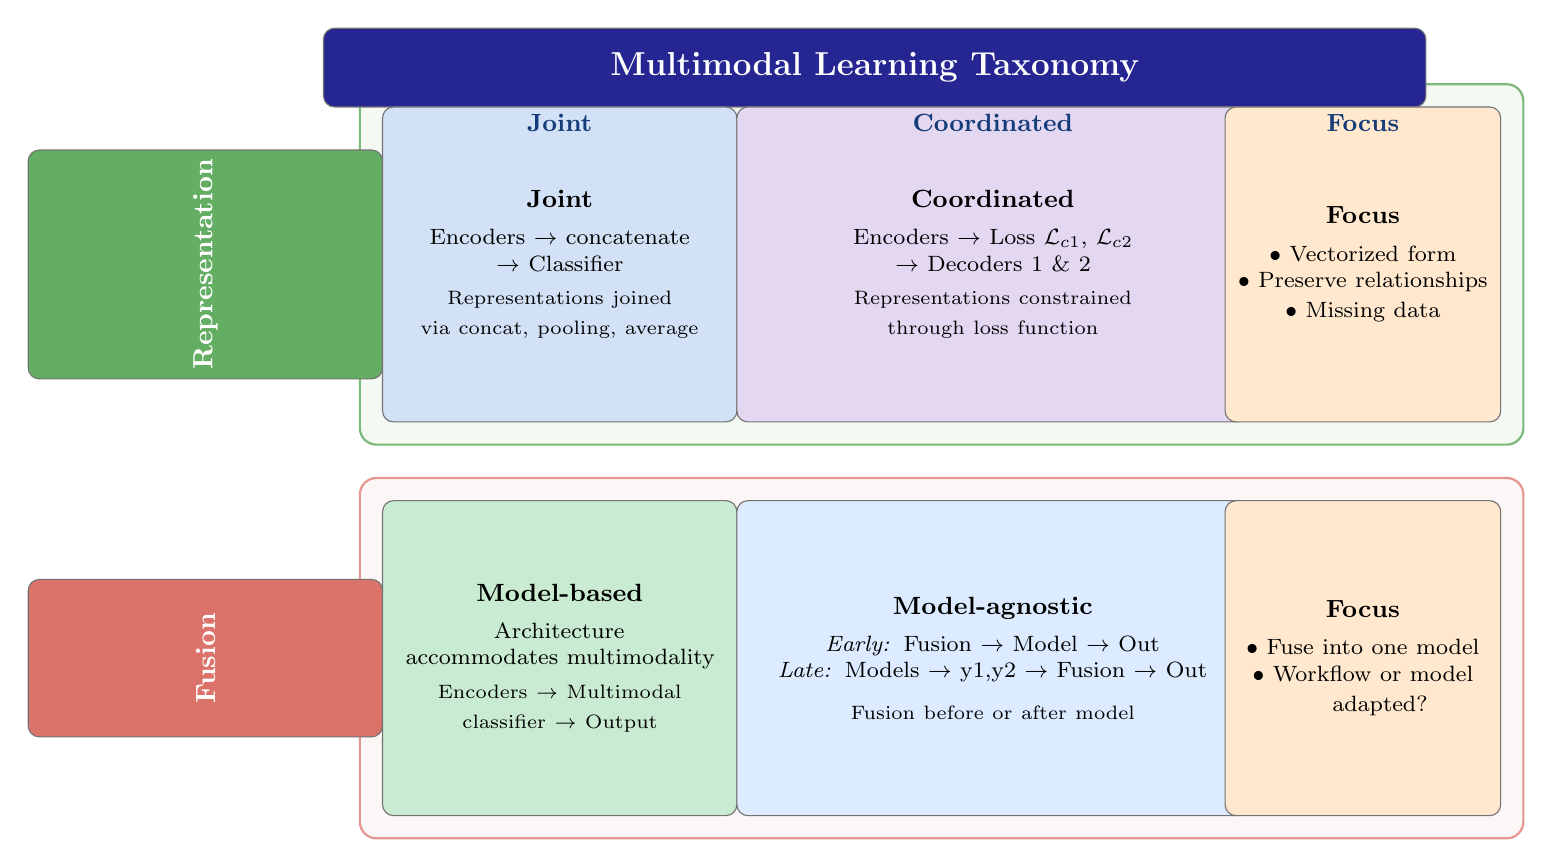
\begin{tikzpicture}[node distance=0.7cm and 1.1cm]
  %% Header row
  \node[basebox,fill=NavyBlue!85,text=white,minimum width=14cm,minimum height=1cm,font=\large\bfseries] (hdr)
      at (0,0) {Multimodal Learning Taxonomy};

  %% Row labels
  \node[basebox,fill=ForestGreen!70,text=white,minimum width=2.0cm,minimum height=4.5cm,
        font=\bfseries,rotate=90,anchor=center] (repLabel) at (-8.5,-2.5) {Representation};
  \node[basebox,fill=coralred!80,text=white,minimum width=2.0cm,minimum height=4.5cm,
        font=\bfseries,rotate=90,anchor=center] (fusLabel) at (-8.5,-7.5) {Fusion};

  %% Representation cells
  \node[basebox,fill=boxblue,minimum width=4.5cm,minimum height=4.0cm,
        text width=4.2cm] (joint) at (-4,-2.5)
      {\textbf{Joint}\\[4pt]
       \footnotesize Encoders $\to$ concatenate\\
       $\to$ Classifier\\[4pt]
       \scriptsize Representations joined\\
       via concat, pooling, average};

  \node[basebox,fill=boxpurple,minimum width=6.5cm,minimum height=4.0cm,
        text width=6.2cm] (coord) at (1.5,-2.5)
      {\textbf{Coordinated}\\[4pt]
       \footnotesize Encoders $\to$ Loss $\mathcal{L}_{c1}$, $\mathcal{L}_{c2}$\\
       $\to$ Decoders 1 \& 2\\[4pt]
       \scriptsize Representations constrained\\
       through loss function};

  \node[basebox,fill=boxorange,minimum width=3.5cm,minimum height=4.0cm,
        text width=3.2cm] (repFocus) at (6.2,-2.5)
      {\textbf{Focus}\\[4pt]
       \footnotesize$\bullet$ Vectorized form\\
       $\bullet$ Preserve relationships\\
       $\bullet$ Missing data};

  %% Fusion cells
  \node[basebox,fill=boxgreen,minimum width=4.5cm,minimum height=4.0cm,
        text width=4.2cm] (modelbased) at (-4,-7.5)
      {\textbf{Model-based}\\[4pt]
       \footnotesize Architecture\\
       accommodates multimodality\\[4pt]
       \scriptsize Encoders $\to$ Multimodal\\
       classifier $\to$ Output};

  \node[basebox,fill=lightblue,minimum width=6.5cm,minimum height=4.0cm,
        text width=6.2cm] (modelagnostic) at (1.5,-7.5)
      {\textbf{Model-agnostic}\\[4pt]
       \footnotesize \textit{Early:} Fusion $\to$ Model $\to$ Out\\
       \textit{Late:} Models $\to$ y1,y2 $\to$ Fusion $\to$ Out\\[4pt]
       \scriptsize Fusion before or after model};

  \node[basebox,fill=boxorange,minimum width=3.5cm,minimum height=4.0cm,
        text width=3.2cm] (fusFocus) at (6.2,-7.5)
      {\textbf{Focus}\\[4pt]
       \footnotesize$\bullet$ Fuse into one model\\
       $\bullet$ Workflow or model\\
       $\quad$ adapted?};

  %% Column headers
  \node[font=\small\bfseries,text=navyblue] at (-4,-0.7) {Joint};
  \node[font=\small\bfseries,text=navyblue] at (1.5,-0.7) {Coordinated};
  \node[font=\small\bfseries,text=navyblue] at (6.2,-0.7) {Focus};

  %% Background containers
  \begin{pgfonlayer}{background}
    \node[rectangle,draw=ForestGreen!60,fill=ForestGreen!5,rounded corners=6pt,thick,
          fit=(joint)(coord)(repFocus),inner sep=8pt] {};
    \node[rectangle,draw=coralred!60,fill=coralred!5,rounded corners=6pt,thick,
          fit=(modelbased)(modelagnostic)(fusFocus),inner sep=8pt] {};
  \end{pgfonlayer}
\end{tikzpicture}
}
\caption{Complete multimodal learning taxonomy. Top row (green): representation strategies. Bottom row (red): fusion strategies. Right column (orange): research focus questions for each row.}
\label{fig:taxonomy_overview}
\end{figure}

\subsection{Representation: Joint Multi-Modal Representations}

Joint representations concatenate (or otherwise pool) modality-specific encodings before a downstream task head. This is the simplest strategy and requires both modalities at training and inference time.

\begin{definition}[Joint Representation]
Given modalities $\mathcal{M} = \{M_1, M_2, \ldots, M_K\}$ with encoder functions $f_k : \mathcal{X}_k \to \R^{d_k}$, the joint representation is:
\[
  \mathbf{r}_{\text{joint}} = \phi\!\left(\mathbf{e}_1, \mathbf{e}_2, \ldots, \mathbf{e}_K\right), \qquad \mathbf{e}_k = f_k(x_k)
\]
where $\phi$ is a pooling function (concatenation, element-wise sum, average, etc.).
\end{definition}

\begin{axiom}[Joint Representation Completeness]
A joint representation is \emph{complete} if $\phi$ is injective with respect to the modality tuple $(\mathbf{e}_1,\ldots,\mathbf{e}_K)$, i.e., distinct modality combinations produce distinct joint representations.
\end{axiom}

\begin{figure}[H]
\centering
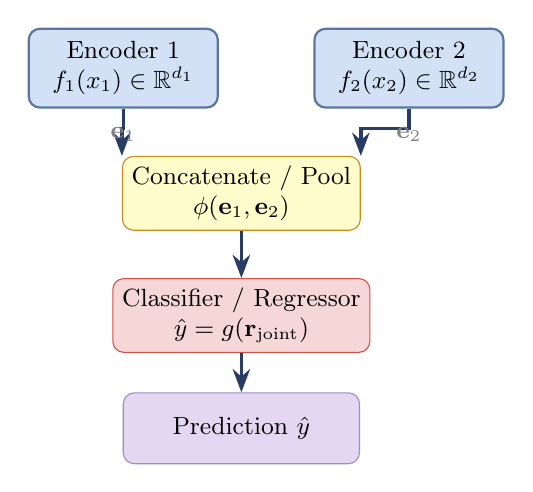
\begin{tikzpicture}[node distance=0.55cm and 0.9cm]
  \node[encnode,minimum width=2.4cm] (enc1) {Encoder 1\\$f_1(x_1) \in \R^{d_1}$};
  \node[encnode,minimum width=2.4cm,right=1.2cm of enc1] (enc2) {Encoder 2\\$f_2(x_2) \in \R^{d_2}$};
  \node[basebox,fill=yellow!20,draw=amber,minimum width=2.4cm,minimum height=0.8cm,
        below=0.6cm of enc1,xshift=1.5cm] (concat) {Concatenate / Pool\\$\phi(\mathbf{e}_1,\mathbf{e}_2)$};
  \node[basebox,fill=boxred,draw=coralred,minimum width=2.4cm,minimum height=0.9cm,
        below=0.6cm of concat] (clf) {Classifier / Regressor\\$\hat{y} = g(\mathbf{r}_{\text{joint}})$};
  \node[outnode,below=0.5cm of clf] (out) {Prediction $\hat{y}$};

  \draw[thickarr] (enc1.south) -- ++(0,-0.25) -| (concat.north west);
  \draw[thickarr] (enc2.south) -- ++(0,-0.25) -| (concat.north east);
  \draw[thickarr] (concat) -- (clf);
  \draw[thickarr] (clf) -- (out);

  \node[font=\small\itshape,color=gray,below=0.12cm of enc1] {$\mathbf{e}_1$};
  \node[font=\small\itshape,color=gray,below=0.12cm of enc2] {$\mathbf{e}_2$};
\end{tikzpicture}
\caption{Joint representation architecture: modality encodings are concatenated and fed to a shared downstream head.}
\label{fig:joint_repr}
\end{figure}

\begin{algorithm}[H]
\caption{Joint Multimodal Representation (Concatenation)}
\label{alg:joint_repr}
\begin{algorithmic}[1]
\Require Modality inputs $\{x_1, x_2, \ldots, x_K\}$, trained encoders $\{f_1,\ldots,f_K\}$,\\
         pooling function $\phi$, downstream head $g_\theta$
\Ensure Prediction $\hat{y}$, joint representation $\mathbf{r}$
\State \textbf{// Step 1: Encode each modality independently}
\For{$k = 1$ to $K$}
  \State $\mathbf{e}_k \gets f_k(x_k)$ \Comment{No gradient if encoder frozen}
\EndFor
\State \textbf{// Step 2: Pool representations}
\State $\mathbf{r}_{\text{joint}} \gets \phi(\mathbf{e}_1, \mathbf{e}_2, \ldots, \mathbf{e}_K)$
  \Comment{e.g., concat: $\mathbf{r} \in \R^{\sum_k d_k}$}
\State \textbf{// Step 3: Downstream task}
\State $\hat{y} \gets g_\theta(\mathbf{r}_{\text{joint}})$
\State \textbf{// Step 4 (training only): Compute loss and update $\theta$}
\If{training}
  \State $\mathcal{L} \gets \ell(\hat{y}, y)$ \Comment{Task-specific loss}
  \State $\theta \gets \theta - \eta\,\nabla_\theta \mathcal{L}$
\EndIf
\State \Return $(\hat{y},\; \mathbf{r}_{\text{joint}})$
\end{algorithmic}
\end{algorithm}

\begin{theorem}[Expressiveness of Concatenation]
Concatenation $\phi_{\text{cat}}(\mathbf{e}_1,\ldots,\mathbf{e}_K) = [\mathbf{e}_1;\ldots;\mathbf{e}_K] \in \R^{\sum_k d_k}$ is the maximal-rank pooling: a linear head $g_\theta$ with $g_\theta(\mathbf{r}) = W\mathbf{r} + b$ can learn arbitrary linear combinations of all modality features, while element-wise sum $\phi_{\text{sum}}$ constrains all $d_k$ to be equal and loses cross-modality interaction terms.
\end{theorem}

\begin{tcolorbox}[laymanbox]
Joint representation is like asking three experts (text analyst, audio analyst, image analyst) to each submit their report, then stapling all reports together before a judge makes the final decision. The judge sees all information simultaneously and can use any combination of the experts' findings.
\end{tcolorbox}

\subsection{Representation: Coordinated Multimodal Representations}

Coordinated representations learn modality-specific encodings that are \emph{aligned through a loss function}, without explicit concatenation. Each modality retains its own representation space; constraints are imposed geometrically (e.g., cosine similarity must be high for matching pairs).

\begin{definition}[Coordinated Representation via Contrastive Loss]
For modalities $M_1, M_2$ with encoders $f_1, f_2$ and a set of positive pairs $\mathcal{P} = \{(x_1^{(i)}, x_2^{(i)})\}_{i=1}^N$, coordinated learning minimises:
\[
  \mathcal{L}_{\text{coord}} = \mathcal{L}_{c1} + \mathcal{L}_{c2}
\]
\[
  \mathcal{L}_{c1} = -\frac{1}{B}\sum_{i=1}^B \log\frac{\exp(\mathbf{e}_1^{(i)} \cdot \mathbf{e}_2^{(i)} / \tau)}{\sum_{j=1}^B \exp(\mathbf{e}_1^{(i)} \cdot \mathbf{e}_2^{(j)} / \tau)}, \quad \mathcal{L}_{c2} = -\frac{1}{B}\sum_{j=1}^B \log\frac{\exp(\mathbf{e}_2^{(j)} \cdot \mathbf{e}_1^{(j)} / \tau)}{\sum_{i=1}^B \exp(\mathbf{e}_2^{(j)} \cdot \mathbf{e}_1^{(i)} / \tau)}
\]
so that matching pairs are geometrically \emph{coordinated} on the shared embedding space.
\end{definition}

\begin{figure}[H]
\centering
\resizebox{\textwidth}{!}{%
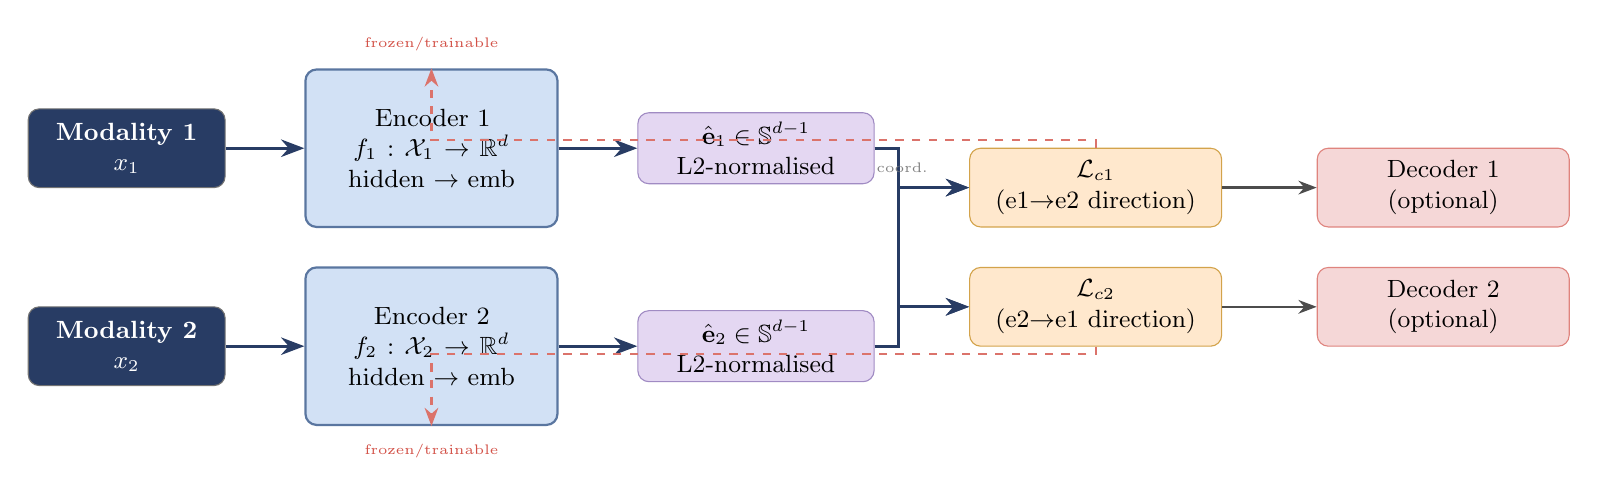
\begin{tikzpicture}[node distance=0.6cm and 0.8cm]
  %% Inputs
  \node[inputnode,minimum width=2.5cm] (m1) {Modality 1\\$x_1$};
  \node[inputnode,minimum width=2.5cm,below=1.5cm of m1] (m2) {Modality 2\\$x_2$};

  %% Encoders (multi-layer indication)
  \node[encnode,right=1.0cm of m1,minimum height=2.0cm,text width=2.5cm] (enc1)
      {Encoder 1\\$f_1: \mathcal{X}_1 \to \R^d$\\hidden $\to$ emb};
  \node[encnode,right=1.0cm of m2,minimum height=2.0cm,text width=2.5cm] (enc2)
      {Encoder 2\\$f_2: \mathcal{X}_2 \to \R^d$\\hidden $\to$ emb};

  %% Projected embeddings
  \node[outnode,right=1.0cm of enc1] (e1) {$\hat{\mathbf{e}}_1 \in \Sph^{d-1}$\\L2-normalised};
  \node[outnode,right=1.0cm of enc2] (e2) {$\hat{\mathbf{e}}_2 \in \Sph^{d-1}$\\L2-normalised};

  %% Loss nodes
  \node[lossnode,right=1.2cm of e1,yshift=-0.5cm] (lc1) {$\mathcal{L}_{c1}$\\(e1$\to$e2 direction)};
  \node[lossnode,below=0.5cm of lc1] (lc2) {$\mathcal{L}_{c2}$\\(e2$\to$e1 direction)};

  %% Decoders / output
  \node[gennode,right=1.2cm of lc1] (dec1) {Decoder 1\\(optional)};
  \node[gennode,right=1.2cm of lc2] (dec2) {Decoder 2\\(optional)};

  %% Arrows
  \draw[thickarr] (m1) -- (enc1);
  \draw[thickarr] (m2) -- (enc2);
  \draw[thickarr] (enc1) -- (e1);
  \draw[thickarr] (enc2) -- (e2);
  \draw[thickarr] (e1.east) -- ++(0.3,0) |- (lc1.west);
  \draw[thickarr] (e2.east) -- ++(0.3,0) |- (lc1.west);
  \draw[thickarr] (e2.east) -- ++(0.3,0) |- (lc2.west);
  \draw[thickarr] (e1.east) -- ++(0.3,0) |- (lc2.west);
  \draw[redarr,dashed] (lc1) -- ++(0,0.6) -| (enc1.north);
  \draw[redarr,dashed] (lc2) -- ++(0,-0.6) -| (enc2.south);
  \draw[arr] (lc1.east) -- (dec1.west);
  \draw[arr] (lc2.east) -- (dec2.west);

  %% Labels
  \node[font=\tiny,color=gray] at ($(e1)!0.5!(lc1)+(-0.3,0)$) {coord.};
  \node[font=\tiny,color=coralred,above=0.1cm of enc1] {frozen/trainable};
  \node[font=\tiny,color=coralred,below=0.1cm of enc2] {frozen/trainable};
\end{tikzpicture}
}
\caption{Coordinated representation: encoders learn geometrically aligned embeddings through dual contrastive losses $\mathcal{L}_{c1}$ and $\mathcal{L}_{c2}$.}
\label{fig:coordinated_repr}
\end{figure}

\begin{algorithm}[H]
\caption{Coordinated Representation Learning (Symmetric Contrastive)}
\label{alg:coord_repr}
\begin{algorithmic}[1]
\Require Paired dataset $\mathcal{D} = \{(x_1^{(i)}, x_2^{(i)})\}_{i=1}^N$; encoders $f_1, f_2$; temperature $\tau$
\Ensure Coordinated encoders mapping both modalities to shared $\Sph^{d-1}$
\For{each mini-batch $\mathcal{B} = \{(x_1^{(i)}, x_2^{(i)})\}_{i=1}^B$}
  \State \textbf{// Encode both modalities}
  \State $\mathbf{e}_1^{(i)} \gets f_1(x_1^{(i)}), \quad \hat{\mathbf{e}}_1^{(i)} \gets \mathbf{e}_1^{(i)}/\Norm{\mathbf{e}_1^{(i)}}$ for $i=1\ldots B$
  \State $\mathbf{e}_2^{(i)} \gets f_2(x_2^{(i)}), \quad \hat{\mathbf{e}}_2^{(i)} \gets \mathbf{e}_2^{(i)}/\Norm{\mathbf{e}_2^{(i)}}$ for $i=1\ldots B$
  \State \textbf{// Compute similarity matrix} $S \in \R^{B \times B}$
  \State $S_{ij} \gets \hat{\mathbf{e}}_1^{(i)} \cdot \hat{\mathbf{e}}_2^{(j)} / \tau$
  \State \textbf{// Loss $\mathcal{L}_{c1}$: Modality-1-to-Modality-2 direction}
  \State $\mathcal{L}_{c1} \gets -\frac{1}{B}\sum_{i=1}^B\log\frac{\exp(S_{ii})}{\sum_{j=1}^B \exp(S_{ij})}$
  \State \textbf{// Loss $\mathcal{L}_{c2}$: Modality-2-to-Modality-1 direction}
  \State $\mathcal{L}_{c2} \gets -\frac{1}{B}\sum_{j=1}^B\log\frac{\exp(S_{jj})}{\sum_{i=1}^B \exp(S_{ij})}$
  \State \textbf{// Combined coordinating loss}
  \State $\mathcal{L}_{\text{coord}} \gets \frac{1}{2}(\mathcal{L}_{c1} + \mathcal{L}_{c2})$
  \State $\mathcal{L}_{\text{coord}}.\text{backward}()$; step optimiser
\EndFor
\end{algorithmic}
\end{algorithm}

\begin{lemma}[Coordinated vs.\ Joint Representations]
Coordinated representations require both modalities only during training (for the loss signal), not necessarily at inference. If $f_1$ encodes text and $f_2$ encodes images, a query may be issued via text alone and matched against pre-encoded image embeddings in the shared space. Joint representations require all modalities at inference.
\end{lemma}

\begin{tcolorbox}[laymanbox]
Coordinated representation is like teaching two translators (one speaking English, one speaking French) to describe the same picture so that similar pictures receive similar descriptions in both languages. The coordination loss measures whether the English and French descriptions are geometrically ``pointing in the same direction'' in a shared semantic space.
\end{tcolorbox}

\subsection{Representation: Handling Missing Modalities}

\begin{definition}[Missing Modality Problem]
A sample $\mathbf{x} = (x_1, x_2, \ldots, x_K)$ has a \emph{missing modality} $M_k$ if $x_k$ is unavailable at inference time. The system must produce a valid prediction using only the available modality subset $\mathcal{A} \subseteq \{1,\ldots,K\}$.
\end{definition}

\begin{axiom}[Zero-Vector Missing Modality Axiom]
\label{ax:missing}
If modality $M_k$ is absent, substituting $\mathbf{e}_k = \bm{0} \in \R^{d_k}$ in a linear projection layer results in zero contribution: $W_k \bm{0} = \bm{0}$. This provides graceful degradation without injecting noise.
\end{axiom}

\begin{algorithm}[H]
\caption{Missing-Modality Robust Inference}
\label{alg:missing_modal}
\begin{algorithmic}[1]
\Require Available modalities $\mathcal{A} \subseteq \{1,\ldots,K\}$; missing modalities $\mathcal{M} = \{1,\ldots,K\}\setminus\mathcal{A}$
\Require Projection weights $\{W_k\}$; fusion function $\phi$
\Ensure Robust representation $\mathbf{r}$
\For{$k = 1$ to $K$}
  \If{$k \in \mathcal{A}$}
    \State $\mathbf{e}_k \gets f_k(x_k)$ \Comment{Standard encoding}
    \State $\hat{\mathbf{e}}_k \gets \mathbf{e}_k / \Norm{\mathbf{e}_k}$ \Comment{L2-normalise}
  \Else
    \State $\hat{\mathbf{e}}_k \gets \bm{0}^d$ \Comment{Zero-token for missing modality (Axiom~\ref{ax:missing})}
  \EndIf
\EndFor
\State $\mathbf{r} \gets \phi(\hat{\mathbf{e}}_1, \ldots, \hat{\mathbf{e}}_K)$ \Comment{Pool only available signals}
\If{all $k \notin \mathcal{A}$}
  \State \Return \textsc{UncertaintyResponse}() \Comment{All modalities missing}
\EndIf
\State \Return $\mathbf{r}$
\end{algorithmic}
\end{algorithm}

\begin{theorem}[Graceful Degradation]
Under the zero-vector substitution of Axiom~\ref{ax:missing}, a $K$-modality fusion model operating on $|\mathcal{A}| = K - m$ available modalities ($m$ missing) achieves performance at least as good as an $(K-m)$-modality model trained from scratch, if the shared embedding space is sufficiently regularised via contrastive learning.
\end{theorem}

\subsection{Fusion: Model-Based Multimodal Fusion}

Model-based fusion integrates multimodal reasoning \emph{within the model architecture} itself — the model is designed so its internal representations simultaneously represent multiple modalities.

\begin{definition}[Model-Based Fusion]
In model-based fusion, the joint prediction arises from a single model $\pi_\Theta : \mathcal{X}_1 \times \cdots \times \mathcal{X}_K \to \mathcal{Y}$ that receives all modalities as input and produces the output via a unified computational graph:
\[
  \hat{y} = \pi_\Theta(x_1, x_2, \ldots, x_K)
\]
The model architecture itself (e.g., cross-modal attention) is what enables multimodal reasoning.
\end{definition}

\begin{figure}[H]
\centering
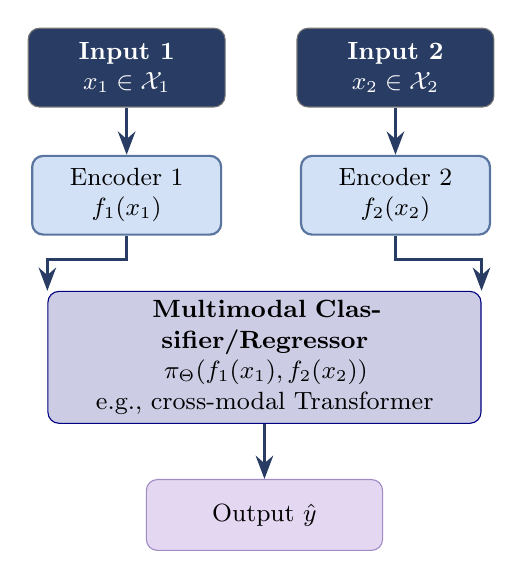
\begin{tikzpicture}[node distance=0.6cm and 0.9cm]
  \node[inputnode,minimum width=2.5cm] (i1) {Input 1\\$x_1 \in \mathcal{X}_1$};
  \node[inputnode,minimum width=2.5cm,right=0.9cm of i1] (i2) {Input 2\\$x_2 \in \mathcal{X}_2$};
  \node[encnode,minimum width=2.4cm,below=0.6cm of i1] (e1) {Encoder 1\\$f_1(x_1)$};
  \node[encnode,minimum width=2.4cm,below=0.6cm of i2] (e2) {Encoder 2\\$f_2(x_2)$};
  \node[basebox,fill=NavyBlue!20,draw=NavyBlue,minimum width=5.5cm,minimum height=1.2cm,
        below=0.7cm of e1,xshift=1.75cm,text width=5.2cm] (clf)
      {\textbf{Multimodal Classifier/Regressor}\\
       $\pi_\Theta(f_1(x_1), f_2(x_2))$\\
       e.g., cross-modal Transformer};
  \node[outnode,below=0.7cm of clf] (out) {Output $\hat{y}$};

  \draw[thickarr] (i1)--(e1);
  \draw[thickarr] (i2)--(e2);
  \draw[thickarr] (e1.south) -- ++(0,-0.3) -| (clf.north west);
  \draw[thickarr] (e2.south) -- ++(0,-0.3) -| (clf.north east);
  \draw[thickarr] (clf)--(out);
\end{tikzpicture}
\caption{Model-based multimodal fusion: the model architecture itself is multimodal-aware.}
\label{fig:model_based_fusion}
\end{figure}

\begin{algorithm}[H]
\caption{Model-Based Multimodal Fusion (Cross-Modal Transformer)}
\label{alg:model_based_fusion}
\begin{algorithmic}[1]
\Require Modality embeddings $\{\hat{\mathbf{e}}_k\}_{k=1}^K$, each $\in \R^d$; Transformer parameters $\Theta$
\Ensure Fused representation $\mathbf{r}_{\text{fused}} \in \R^d$
\State \textbf{// Step 1: Build modality token sequence}
\State $X \gets \text{stack}([\hat{\mathbf{e}}_1, \hat{\mathbf{e}}_2, \ldots, \hat{\mathbf{e}}_K],\; \text{dim}=1)$ \Comment{$[B, K, d]$}
\State \textbf{// Step 2: Add learnable modality positional encodings}
\State $X \gets X + P$ \Comment{$P \in \R^{K \times d}$ learned modality tags}
\State \textbf{// Step 3: Self-attention across modalities (2 layers, Pre-LN)}
\For{layer $\ell = 1$ to $L$}
  \State $X \gets X + \MHA(\LN(X))$ \Comment{Cross-modal attention residual}
  \State $X \gets X + \text{FFN}(\LN(X))$ \Comment{Position-wise FFN residual}
\EndFor
\State \textbf{// Step 4: Mean-pool over modality tokens}
\State $\mathbf{r}_{\text{fused}} \gets \frac{1}{K}\sum_{k=1}^K X_{:,k,:}$ \Comment{$[B, d]$}
\State \textbf{// Step 5: Regression / classification head}
\State $\hat{y} \gets g_\theta(\mathbf{r}_{\text{fused}})$
\State \Return $(\hat{y}, \mathbf{r}_{\text{fused}})$
\end{algorithmic}
\end{algorithm}

\begin{theorem}[Cross-Modal Attention Expressiveness]
Multi-head attention with $h$ heads over $K$ modality tokens learns $h$ independent linear combinations of modality interactions. For $K=3$ modalities and $h=8$ heads, each head can specialise in a distinct pairwise relationship (text-audio, audio-video, text-video) plus their higher-order combinations, without manual feature engineering.
\end{theorem}

\subsection{Fusion: Model-Agnostic Early Fusion}

Early fusion combines raw or modestly-encoded features \emph{before} passing them into the main model.

\begin{definition}[Early Fusion]
In early fusion, features from all modalities are combined into a single representation $\mathbf{z} = \phi_{\text{early}}(x_1, x_2, \ldots, x_K)$ before any learned model is applied:
\[
  \hat{y} = g_\theta(\phi_{\text{early}}(x_1, \ldots, x_K))
\]
The model $g_\theta$ sees only the fused feature; it is unaware of which features originated from which modality.
\end{definition}

\begin{figure}[H]
\centering
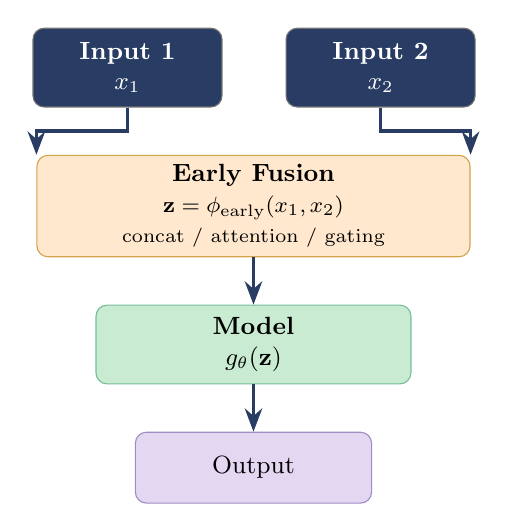
\begin{tikzpicture}[node distance=0.6cm and 1.0cm]
  \node[inputnode,minimum width=2.4cm] (i1) {Input 1\\$x_1$};
  \node[inputnode,minimum width=2.4cm,right=0.8cm of i1] (i2) {Input 2\\$x_2$};
  \node[lossnode,minimum width=5.5cm,below=0.6cm of i1,xshift=1.6cm] (fuse)
      {\textbf{Early Fusion}\\\footnotesize$\mathbf{z} = \phi_{\text{early}}(x_1, x_2)$\\\scriptsize concat / attention / gating};
  \node[retnode,minimum width=4.0cm,below=0.6cm of fuse] (model)
      {\textbf{Model}\\$g_\theta(\mathbf{z})$};
  \node[outnode,below=0.6cm of model] (out) {Output};

  \draw[thickarr] (i1.south) -- ++(0,-0.3) -| (fuse.north west);
  \draw[thickarr] (i2.south) -- ++(0,-0.3) -| (fuse.north east);
  \draw[thickarr] (fuse)--(model);
  \draw[thickarr] (model)--(out);
\end{tikzpicture}
\caption{Model-agnostic early fusion: modalities are merged before any deep model processing.}
\label{fig:early_fusion}
\end{figure}

\begin{algorithm}[H]
\caption{Model-Agnostic Early Fusion}
\label{alg:early_fusion}
\begin{algorithmic}[1]
\Require Raw modality inputs $\{x_k\}_{k=1}^K$; optional shallow encoders $\{h_k\}$
\Require Fusion function $\phi_{\text{early}}$; deep model $g_\theta$
\Ensure Prediction $\hat{y}$
\State \textbf{// Step 1: Shallow encoding (optional, e.g., spectrogram, normalisation)}
\For{$k = 1$ to $K$}
  \State $\tilde{x}_k \gets h_k(x_k)$ \Comment{e.g., MFCC extraction, frame resizing}
\EndFor
\State \textbf{// Step 2: Early fusion}
\State $\mathbf{z} \gets \phi_{\text{early}}(\tilde{x}_1, \ldots, \tilde{x}_K)$ \Comment{e.g., concatenation along feature axis}
\State \textbf{// Step 3: Single deep model processes fused input}
\State $\hat{y} \gets g_\theta(\mathbf{z})$
\State \Return $\hat{y}$
\end{algorithmic}
\end{algorithm}

\begin{lemma}[Early Fusion Trade-off]
Early fusion achieves the lowest inference latency (single forward pass through $g_\theta$) but requires all modalities to be present and aligned. Missing modalities cannot be trivially handled without imputation, unlike coordinated or late fusion architectures.
\end{lemma}

\subsection{Fusion: Model-Agnostic Late Fusion}

Late fusion processes each modality through an independent model and combines their predictions.

\begin{definition}[Late Fusion]
In late fusion, $K$ independent models $\{g_k\}_{k=1}^K$ each produce a prediction $\hat{y}_k = g_k(x_k)$. A fusion function $\phi_{\text{late}}$ combines these predictions:
\[
  \hat{y} = \phi_{\text{late}}(\hat{y}_1, \hat{y}_2, \ldots, \hat{y}_K)
\]
Common choices: $\phi_{\text{late}} = $ mean, weighted mean, learned combiner (linear, MLP).
\end{definition}

\begin{figure}[H]
\centering
\resizebox{0.9\textwidth}{!}{%
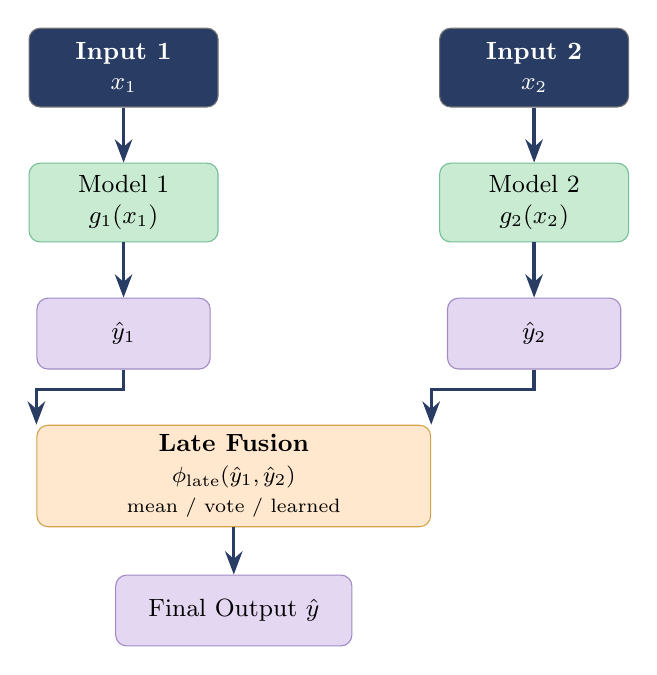
\begin{tikzpicture}[node distance=0.6cm and 1.0cm]
  \node[inputnode,minimum width=2.4cm] (i1) {Input 1\\$x_1$};
  \node[inputnode,minimum width=2.4cm,right=2.8cm of i1] (i2) {Input 2\\$x_2$};
  \node[retnode,minimum width=2.4cm,below=0.7cm of i1] (m1) {Model 1\\$g_1(x_1)$};
  \node[retnode,minimum width=2.4cm,below=0.7cm of i2] (m2) {Model 2\\$g_2(x_2)$};
  \node[outnode,minimum width=2.2cm,below=0.7cm of m1] (y1) {$\hat{y}_1$};
  \node[outnode,minimum width=2.2cm,below=0.7cm of m2] (y2) {$\hat{y}_2$};
  \node[lossnode,minimum width=5.0cm,below=0.7cm of y1,xshift=1.4cm] (fuse)
      {\textbf{Late Fusion}\\\footnotesize$\phi_{\text{late}}(\hat{y}_1, \hat{y}_2)$\\\scriptsize mean / vote / learned};
  \node[outnode,minimum width=3.0cm,below=0.6cm of fuse] (out) {Final Output $\hat{y}$};

  \draw[thickarr] (i1)--(m1); \draw[thickarr] (i2)--(m2);
  \draw[thickarr] (m1)--(y1); \draw[thickarr] (m2)--(y2);
  \draw[thickarr] (y1.south) -- ++(0,-0.25) -| (fuse.north west);
  \draw[thickarr] (y2.south) -- ++(0,-0.25) -| (fuse.north east);
  \draw[thickarr] (fuse)--(out);
\end{tikzpicture}
}
\caption{Model-agnostic late fusion: independent modality models produce predictions that are combined downstream.}
\label{fig:late_fusion}
\end{figure}

\begin{algorithm}[H]
\caption{Model-Agnostic Late Fusion (Weighted Average)}
\label{alg:late_fusion}
\begin{algorithmic}[1]
\Require Inputs $\{x_k\}_{k=1}^K$; independent models $\{g_k\}_{k=1}^K$; weights $\{w_k\}$ with $\sum_k w_k = 1$
\Ensure Final prediction $\hat{y}$
\For{$k = 1$ to $K$}
  \State $\hat{y}_k \gets g_k(x_k)$ \Comment{Independent modality prediction}
\EndFor
\State \textbf{// Weighted late fusion}
\State $\hat{y} \gets \sum_{k=1}^K w_k \hat{y}_k$
\Comment{Alternatively: majority vote for classification, learned MLP}
\State \Return $\hat{y}$
\end{algorithmic}
\end{algorithm}

\begin{proposition}[Late Fusion Missing-Modality Robustness]
Late fusion is the most robust to missing modalities: if $M_k$ is absent, the weight $w_k$ can be set to zero and the remaining modalities are re-normalised: $\hat{y} = \frac{\sum_{k \in \mathcal{A}} w_k \hat{y}_k}{\sum_{k \in \mathcal{A}} w_k}$, requiring no architectural changes.
\end{proposition}

\begin{tcolorbox}[taxonomybox,title={Taxonomy Summary for MIVA-KNIGHT}]
\begin{tabular}{lll}
\toprule
\textbf{Category} & \textbf{Type} & \textbf{MIVA-KNIGHT Instance} \\
\midrule
Representation & Joint & Pipeline A/B: fused BERT+ResNet embedding \\
Representation & Coordinated & Pipelines A–D: InfoNCE/SupCon losses \\
Representation & Missing data & Axiom~\ref{ax:missing}: zero-vector substitution \\
Fusion & Model-based & Pipeline E: Cross-modal Transformer \\
Fusion & Early & Pipelines A/B: stacked modality tokens \\
Fusion & Late & Inference: domain-specialised FAISS + KG \\
\bottomrule
\end{tabular}
\end{tcolorbox}

%%
%% ============================================================
%% PART III — MATHEMATICAL FOUNDATIONS
%% ============================================================
%%
\newpage
\section{Mathematical Foundations}
\label{sec:math}

\subsection{The Shared Unit Hypersphere}

\begin{definition}[Unit Hypersphere $\Sph^{511}$]
The shared embedding space is the $(512{-}1)$-dimensional unit hypersphere:
\[
  \Sph^{511} = \left\{v \in \R^{512} \;\Big|\; \Norm{v} = 1\right\}.
\]
All modality encoders project their outputs to $\Sph^{511}$ via L2-normalisation.
\end{definition}

\begin{axiom}[Shared Metric Space Alignment]
All modal encoders $(f_T, f_I, f_A)$ are trained so that:
\[
  \Norm{f_T(x_T)}_2 = \Norm{f_I(x_I)}_2 = \Norm{f_A(x_A)}_2 = 1, \quad
  \cos(u,v) = u \cdot v \quad \forall\; u,v \in \Sph^{511}.
\]
\end{axiom}

\begin{axiom}[Domain-Agnostic Shared Space]
\label{ax:shared}
The shared encoder weights
$W_{\text{shared}} = \{W_{\text{TextProj}}, W_{\text{AudioProj}}, W_{\text{BERT}}, W_{\text{Wav2Vec}}\}$
are identical across domains. Only $(I_{\text{path}}, \KG_{\text{path}}, \text{NER}, \tau)$ differ per domain. This is the central claim: $\Sph^{511}$ is domain-agnostic.
\end{axiom}

\begin{lemma}[Cosine–Dot Product Equivalence]
\label{lem:cosdot}
For any $u, v \in \Sph^{511}$: $\cos(u, v) = u \cdot v$.
\end{lemma}
\begin{proof}
Since $\Norm{u}_2 = \Norm{v}_2 = 1$:
$\cos(u,v) = \frac{u \cdot v}{\Norm{u}_2\,\Norm{v}_2} = \frac{u \cdot v}{1 \cdot 1} = u \cdot v.$ \qed
\end{proof}

\begin{theorem}[Domain Switch Efficiency]
\label{thm:switch}
Under Axiom~\ref{ax:shared}, switching domain requires reloading only the FAISS index ($\approx$1--3\,s) and KG pickle ($\approx$0.5--2\,s), reducing domain-swap latency by a factor of $10$--$20\times$ compared to full model reload ($\approx$50--90\,s for BERT + Wav2Vec).
\end{theorem}

\subsection{Activation Functions and Normalisation}

\begin{definition}[GELU Activation]
\[
  \GELU(x) = x \cdot \Phi(x), \qquad \Phi(x) = \frac{1}{2}\left[1 + \text{erf}\!\left(\frac{x}{\sqrt{2}}\right)\right].
\]
Approximation: $\GELU(x) \approx 0.5x\!\left(1 + \tanh\!\left[\sqrt{\tfrac{2}{\pi}}\left(x + 0.044715x^3\right)\right]\right)$.
\end{definition}

\begin{definition}[Layer Normalisation]
For $x \in \R^d$ with $\mu = \frac{1}{d}\sum_i x_i$, $\sigma^2 = \frac{1}{d}\sum_i (x_i - \mu)^2$:
\[
  \LN(x) = \gamma \odot \frac{x - \mu}{\sqrt{\sigma^2 + \varepsilon}} + \beta, \quad \varepsilon = 10^{-5},\; \gamma, \beta \in \R^d \text{ learned.}
\]
\end{definition}

\begin{lemma}[GELU vs. ReLU]
$\text{ReLU}(x) = \max(0,x)$ has zero gradient for $x < 0$ (dead neuron). $\GELU$ is smooth and non-zero everywhere, providing continuous gradients — critical for embedding learning.
\end{lemma}

\subsection{Projection Networks}

\begin{definition}[General Projection MLP]
\label{def:projmlp}
For input $x \in \R^{d_{\text{in}}}$, the projection head $f_\theta : \R^{d_{\text{in}}} \to \Sph^{511}$ is:
\[
  h_1 = W_1 x + b_1 \in \R^{d_{\text{in}}}, \quad h_2 = \GELU(h_1), \quad h_3 = \LN(h_2)
\]
\[
  h_4 = W_2 h_3 + b_2 \in \R^{512}, \quad h_5 = \LN(h_4), \quad \hat{e} = h_5 / \Norm{h_5}_2 \in \Sph^{511}
\]
where $W_1 \in \R^{d_{\text{in}} \times d_{\text{in}}}$, $W_2 \in \R^{512 \times d_{\text{in}}}$.
\end{definition}

%%
%% ============================================================
%% PART IV — PIPELINE A: GENERAL DOMAIN (COCO)
%% ============================================================
%%
\newpage
\section{Pipeline A: General Domain — COCO Text-Image Retrieval}
\label{sec:pipelineA}

\subsection{Overview}

Pipeline~A trains a coordinated multimodal embedding on the COCO val2017 dataset (202,654 image-caption pairs) using symmetric InfoNCE loss, building the foundation for the shared $\Sph^{511}$ space.

\begin{figure}[H]
\centering
\resizebox{\textwidth}{!}{%
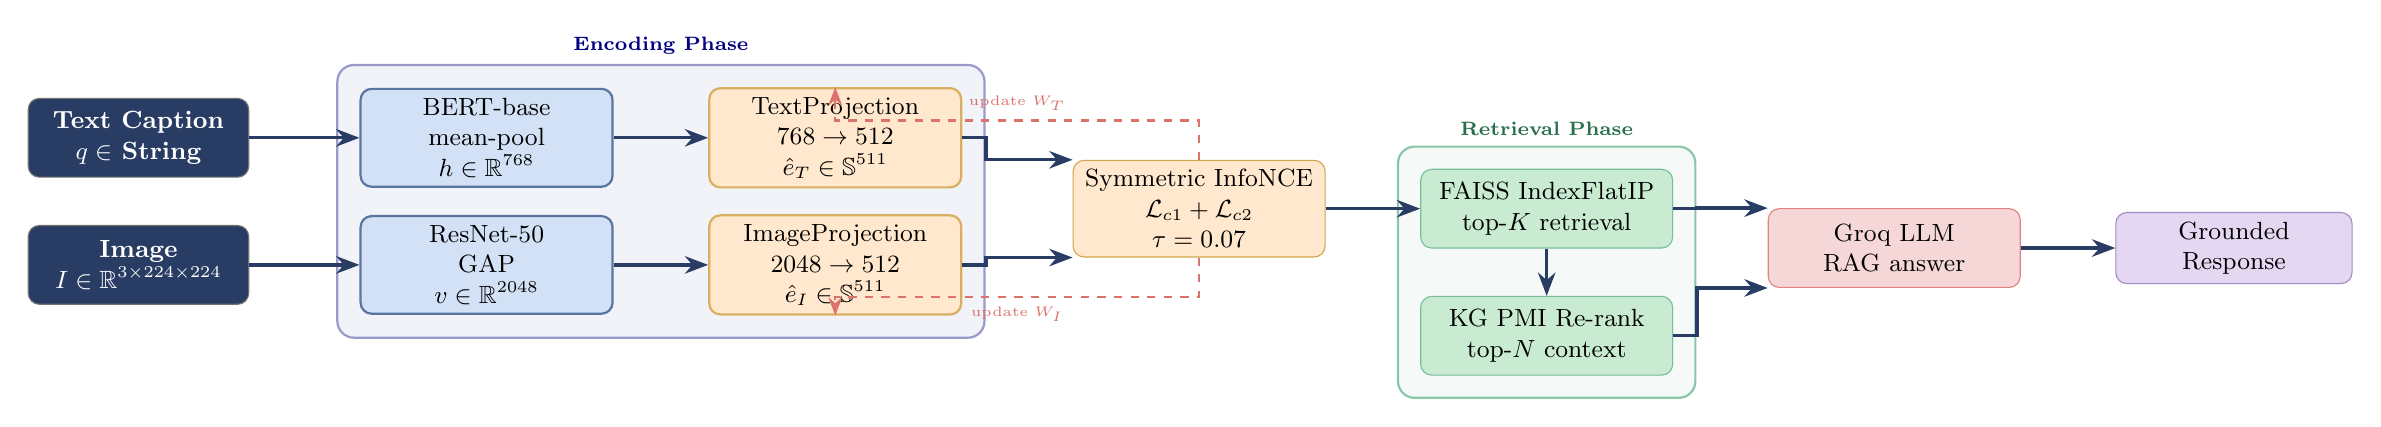
\begin{tikzpicture}[node distance=0.7cm and 1.0cm]
  \node[inputnode] (textq) at (0,0) {Text Caption\\$q \in$ String};
  \node[inputnode,below=0.6cm of textq] (imgq) {Image\\$I \in \R^{3\times224\times224}$};

  \node[encnode,right=1.4cm of textq] (bert) {BERT-base\\mean-pool\\$h \in \R^{768}$};
  \node[encnode,right=1.4cm of imgq] (resnet) {ResNet-50\\GAP\\$v \in \R^{2048}$};

  \node[projnode,right=1.2cm of bert] (tproj) {TextProjection\\$768 \to 512$\\$\hat{e}_T \in \Sph^{511}$};
  \node[projnode,right=1.2cm of resnet] (iproj) {ImageProjection\\$2048 \to 512$\\$\hat{e}_I \in \Sph^{511}$};

  \node[lossnode,right=1.4cm of tproj,yshift=-0.9cm] (loss) {Symmetric InfoNCE\\$\mathcal{L}_{c1} + \mathcal{L}_{c2}$\\$\tau = 0.07$};

  \node[retnode,right=1.2cm of loss] (faiss) {FAISS IndexFlatIP\\top-$K$ retrieval};
  \node[retnode,below=0.6cm of faiss] (kg) {KG PMI Re-rank\\top-$N$ context};
  \node[gennode,right=1.2cm of faiss,yshift=-0.5cm] (llm) {Groq LLM\\RAG answer};
  \node[outnode,right=1.2cm of llm] (out) {Grounded\\Response};

  \draw[thickarr] (textq)--(bert); \draw[thickarr] (imgq)--(resnet);
  \draw[thickarr] (bert)--(tproj); \draw[thickarr] (resnet)--(iproj);
  \draw[thickarr] (tproj.east) -- ++(0.3,0) |- (loss.north west);
  \draw[thickarr] (iproj.east) -- ++(0.3,0) |- (loss.south west);
  \draw[redarr,dashed] (loss.north) -- ++(0,0.5) -| (tproj.north)
      node[near start,above,font=\tiny]{update $W_T$};
  \draw[redarr,dashed] (loss.south) -- ++(0,-0.5) -| (iproj.south)
      node[near start,below,font=\tiny]{update $W_I$};
  \draw[thickarr] (loss.east) -- ++(0.3,0) |- (faiss.west);
  \draw[thickarr] (faiss.south)--(kg.north);
  \draw[thickarr] (faiss.east) -- ++(0.3,0) |- (llm.north west);
  \draw[thickarr] (kg.east) -- ++(0.3,0) |- (llm.south west);
  \draw[thickarr] (llm)--(out);

  \begin{pgfonlayer}{background}
    \node[rectangle,draw=NavyBlue!40,fill=NavyBlue!5,rounded corners=6pt,thick,
          fit=(bert)(resnet)(tproj)(iproj),inner sep=8pt,
          label={[font=\scriptsize\bfseries,color=NavyBlue]above:Encoding Phase}] {};
    \node[rectangle,draw=mintgreen!60,fill=mintgreen!5,rounded corners=6pt,thick,
          fit=(faiss)(kg),inner sep=8pt,
          label={[font=\scriptsize\bfseries,color=mintgreen!70!black]above:Retrieval Phase}] {};
  \end{pgfonlayer}
\end{tikzpicture}
}
\caption{Pipeline~A full architecture: COCO text-image coordinated embedding with two-stage RAG retrieval.}
\label{fig:pipeline_a}
\end{figure}

\subsection{Text Encoder (BERT + TextProjection)}

\begin{algorithm}[H]
\caption{TextEncoderV2.encode — BERT Mean-Pool + TextProjection}
\label{alg:textencode}
\begin{algorithmic}[1]
\Require Text $t \in$ String; frozen BERT; trained TextProjection $P_\theta$ (Def.~\ref{def:projmlp}, $d_{\text{in}}=768$)
\Ensure $e_q \in \Sph^{511}$, entity set $\mathcal{E}_q$, domain hint
\State \textbf{Tokenise:} $\text{tokens} \gets \text{WordPiece}(t, \texttt{max\_length}=128, \texttt{truncation=True})$
\State \textbf{BERT forward} (no grad):
  $H \gets \text{BERT}(\text{tokens}).\text{last\_hidden\_state} \in \R^{1 \times T \times 768}$
\State \textbf{Mean pool:} $h_{\text{BERT}} \gets \frac{1}{T}\sum_{t=1}^T H_{:,t,:} \in \R^{768}$
\State \textbf{Project:} $e_{\text{raw}} \gets P_\theta(h_{\text{BERT}}) \in \R^{512}$
\State \textbf{Normalise:} $e_q \gets e_{\text{raw}} / \Norm{e_{\text{raw}}}_2$
\State \textbf{NER:} $\mathcal{E}_q \gets \{\text{noun chunks}\} \cup \{\text{named entities}\}$ (lowercased)
\State \textbf{Domain detect:} $n_m \gets |\{w \in \textsc{Medical\_Terms} : w \subseteq t.\text{lower}()\}|$
\State domain\_hint $\gets$ ``medical'' if $n_m \ge 2$ else None
\State \Return $(e_q,\; \mathcal{E}_q,\; \text{domain\_hint})$
\end{algorithmic}
\end{algorithm}

\begin{remark}[Mean Pooling vs. CLS]
CLS token ($H_{:,0,:}$) is optimised for classification but degrades for long sequences. Mean pooling ($\frac{1}{T}\sum H_{:,t,:}$) provides better semantic similarity for retrieval tasks (consistent with sentence-transformers literature).
\end{remark}

\subsection{Image Encoder (ResNet-50 + ImageProjection)}

\begin{definition}[ImageProjection $f_\phi$]
\[
  f_\phi : \R^{2048} \to \Sph^{511}, \qquad
  f_\phi(x) = \frac{g_\phi(x)}{\Norm{g_\phi(x)}_2}
\]
\[
  g_\phi(x) = \LN_{512}\!\left(W_2 \cdot \GELU(\LN_{2048}(W_1 x + b_1)) + b_2\right)
\]
where $W_1 \in \R^{2048 \times 2048}$, $W_2 \in \R^{512 \times 2048}$. Total: $\approx$5.25\,M parameters.
\end{definition}

\begin{axiom}[Mandatory ImageNet Normalisation]
Input images must be normalised per channel:
\[
  \hat{x}_{c,h,w} = \frac{x_{c,h,w} - \mu_c}{\sigma_c}, \quad
  \bm{\mu} = [0.485, 0.456, 0.406], \quad \bm{\sigma} = [0.229, 0.224, 0.225].
\]
ResNet-50 BatchNorm layers are calibrated with these statistics; deviations degrade pool5 features.
\end{axiom}

\subsection{InfoNCE Contrastive Loss}

\begin{definition}[Symmetric InfoNCE Loss]
For batch size $B$, positive pairs $\{(\hat{e}_T^{(i)}, \hat{e}_I^{(i)})\}_{i=1}^B$, temperature $\tau = 0.07$:
\[
  S_{ij} = \hat{e}_T^{(i)} \cdot \hat{e}_I^{(j)}, \qquad
  \mathcal{L}_{\text{InfoNCE}} = \frac{1}{2}\left[
    -\frac{1}{B}\sum_i \log\frac{e^{S_{ii}/\tau}}{\sum_j e^{S_{ij}/\tau}}
    -\frac{1}{B}\sum_j \log\frac{e^{S_{jj}/\tau}}{\sum_i e^{S_{ij}/\tau}}
  \right]
\]
\end{definition}

\begin{lemma}[Random Baseline Loss]
At random initialisation, $\mathbb{E}[\mathcal{L}_{\text{InfoNCE}}] = \log B$. For $B = 32$: $\log 32 \approx 3.47$.
\end{lemma}

\begin{algorithm}[H]
\caption{Pipeline A Training Epoch}
\label{alg:trainepoch_A}
\begin{algorithmic}[1]
\Require COCO DataLoader $L$; TextProjection $P_\theta$; ImageProjection $f_\phi$; $\tau = 0.07$
\Ensure Updated $P_\theta, f_\phi$; epoch loss
\State total\_loss $\gets 0$
\ForEach{batch $(I^{B \times 3 \times 224 \times 224},\; T^B)$ in $L$}
  \State $\hat{e}_T^{(b)} \gets \textsc{TextEncoderV2}(T[b])$ for $b=1\ldots B$ \quad $\Rightarrow E_T \in \R^{B \times 512}$
  \State $\hat{e}_I^{(b)} \gets f_\phi(\text{ResNet50}(I[b]))$ for $b=1\ldots B$ \quad $\Rightarrow E_I \in \R^{B \times 512}$
  \State $S \gets E_T \cdot E_I^\top \in \R^{B \times B}$
  \State $\mathcal{L} \gets \mathcal{L}_{\text{InfoNCE}}(E_T, E_I, \tau)$
  \State optimizer.zero\_grad(); $\mathcal{L}$.backward()
  \State clip\_grad\_norm$(\nabla\theta, c=1.0)$
  \State optimizer.step(); scheduler.step()
  \State total\_loss $\mathrel{+}= \mathcal{L}$.item()
\EndFor
\State \Return total\_loss / $|L|$
\end{algorithmic}
\end{algorithm}

%%
%% ============================================================
%% PART V — KNOWLEDGE GRAPH CONSTRUCTION
%% ============================================================
%%
\newpage
\section{Knowledge Graph: PMI-Weighted Entity Graph}
\label{sec:kg}

\begin{definition}[General Knowledge Graph $\KG_G$]
\[
  \KG_G = (\mathcal{V}_G, \mathcal{E}_G, w), \quad
  \mathcal{V}_G = \text{top-2000 COCO entities (spaCy)}, \quad
  (a,b) \in \mathcal{E}_G \Leftrightarrow \text{PMI}(a,b) > 0.
\]
\[
  \text{PMI}(a,b) = \log\frac{c_{ab} \cdot N}{f_a \cdot f_b + \varepsilon}, \quad w(a,b) = \text{PMI}(a,b).
\]
\end{definition}

\begin{axiom}[PMI Semantic Association]
$\text{PMI}(a,b) > 0 \Leftrightarrow$ entities $a, b$ co-occur more than expected under independence.
\end{axiom}

\begin{algorithm}[H]
\caption{Build General NER Knowledge Graph (PMI-Weighted)}
\label{alg:kg_build}
\begin{algorithmic}[1]
\Require $N$ COCO captions; spaCy \texttt{en\_core\_web\_sm}; top-$V = 2000$ entities
\Ensure \texttt{ner\_kg\_general.pkl}: $\text{dict}[\text{entity} \to \text{dict}[\text{entity} \to \text{PMI}]]$
\For{captions in batches of 1,000}
  \State $\mathcal{E}_{\text{doc}} \gets \{\text{noun chunks}\} \cup \{\text{named entities}\}$ (lowercased)
  \State Append $\mathcal{E}_{\text{doc}}$ to all\_doc\_entities
\EndFor
\State entity\_freq $\gets \text{Counter}(\bigcup \mathcal{E}_{\text{doc}})$
\State $\mathcal{V}_G \gets \text{top-}V$ entities with freq $\ge 5$
\For{each document entity set $E_i$ (filtered to $\mathcal{V}_G$)}
  \For{each symmetric pair $(a,b) \in E_i \times E_i,\; a \ne b$}
    \State cooc$[a][b] \mathrel{+}= 1$; cooc$[b][a] \mathrel{+}= 1$
  \EndFor
\EndFor
\For{each $a \in \mathcal{V}_G$ with freq $\ge 5$}
  \For{each $(b, c_{ab})$ with $c_{ab} \ge 3$}
    \State $\text{pmi} \gets \log(c_{ab} \cdot N / (f_a \cdot f_b + \varepsilon))$
    \If{pmi $> 0$} $\KG_G[a][b] \gets \text{pmi}$ \EndIf
  \EndFor
\EndFor
\State \texttt{pickle.dump}($\KG_G$)
\end{algorithmic}
\end{algorithm}

\begin{algorithm}[H]
\caption{KG Depth-First Neighbour Search (max-2-hop)}
\label{alg:kgdfs}
\begin{algorithmic}[1]
\Require Entity $v$, KG $\KG$, max\_hops $= 2$
\Ensure Neighbour list
\State visited $\gets \emptyset$; neighbours $\gets []$
\State \Call{DFS}{$v$, 1}
\Procedure{DFS}{current, hops}
  \If{hops $>$ max\_hops \textbf{or} current $\in$ visited} \Return \EndIf
  \State visited $\gets$ visited $\cup$ \{current\}
  \ForEach{$(h, r, t) \in \KG$.\text{relationships}}
    \If{$h = $ current} neighbours.append$(h, r, t, \text{hops})$; \Call{DFS}{$t$, hops+1} \EndIf
    \If{$t = $ current} neighbours.append$(t, r_{\text{inv}}, h, \text{hops})$; \Call{DFS}{$h$, hops+1} \EndIf
  \EndFor
\EndProcedure
\end{algorithmic}
\end{algorithm}

%%
%% ============================================================
%% PART VI — PIPELINE B: MEDICAL DOMAIN TRANSFER (ROCO)
%% ============================================================
%%
\newpage
\section{Pipeline B: Medical Domain Transfer — ROCO Radiology}
\label{sec:pipelineB}

\subsection{Core Thesis: Surgical Domain Transfer}

\begin{definition}[Domain Transfer]
Let $\Sph^{511}$ be the shared embedding space from Pipeline~A, where TextProjection $f_T$ maps captions. Domain transfer trains $f_I^{\text{ROCO}}$ such that:
\[
  f_I^{\text{ROCO}}\!\left(\text{ResNet}(\text{X-ray}_i)\right) \approx f_T(\text{caption}_i), \quad \forall i \in \text{ROCO train},
\]
without moving existing text embeddings.
\end{definition}

\begin{theorem}[Surgical Transfer Efficiency]
\label{thm:efficiency}
Pipeline~B modifies only $5.25\,\text{M}$ out of $235.15\,\text{M}$ total parameters:
\[
  \text{Efficiency} = \frac{5.25}{235.15} \approx 2.23\%.
\]
\end{theorem}

\begin{figure}[H]
\centering
\resizebox{0.9\textwidth}{!}{%
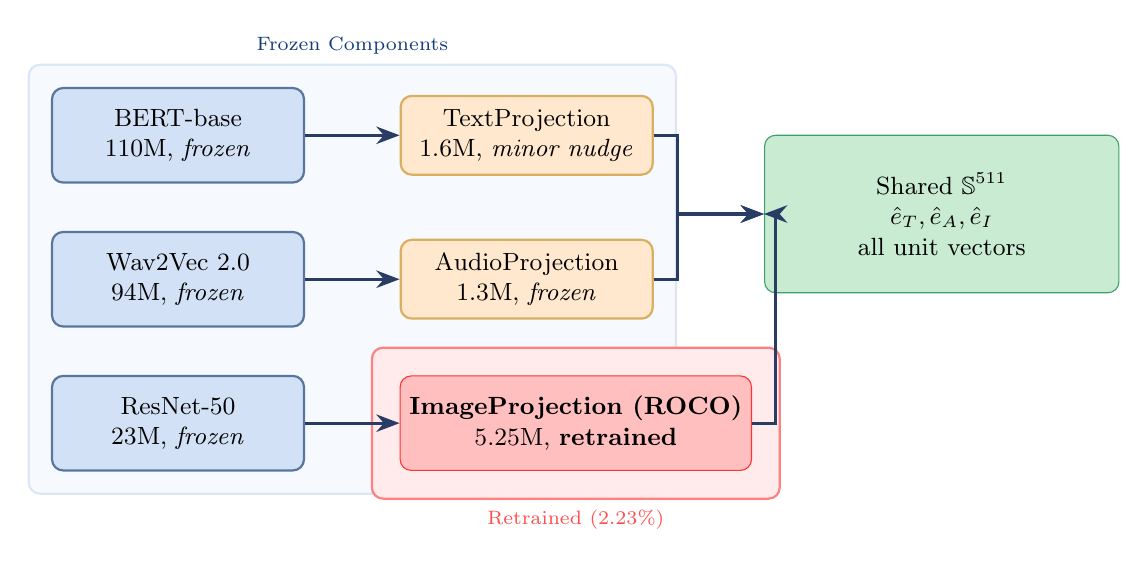
\begin{tikzpicture}[node distance=0.6cm and 1.0cm]
  %% Frozen components
  \node[encnode,minimum width=3.2cm,minimum height=1.2cm] (bert) {BERT-base\\110M, \textit{frozen}};
  \node[encnode,minimum width=3.2cm,minimum height=1.2cm,below=0.6cm of bert] (wav2vec) {Wav2Vec 2.0\\94M, \textit{frozen}};
  \node[encnode,minimum width=3.2cm,minimum height=1.2cm,below=0.6cm of wav2vec] (resnet) {ResNet-50\\23M, \textit{frozen}};

  \node[projnode,minimum width=3.2cm,right=1.2cm of bert] (tproj) {TextProjection\\1.6M, \textit{minor nudge}};
  \node[projnode,minimum width=3.2cm,right=1.2cm of wav2vec] (aproj) {AudioProjection\\1.3M, \textit{frozen}};
  \node[basebox,fill=red!25,draw=red!80,minimum width=3.2cm,minimum height=1.2cm,
        right=1.2cm of resnet] (iproj) {\textbf{ImageProjection (ROCO)}\\5.25M, \textbf{retrained}};

  \node[basebox,fill=boxgreen,draw=mintgreen,minimum width=4.5cm,minimum height=2.0cm,
        right=1.4cm of tproj,yshift=-1.0cm] (shared) {Shared $\Sph^{511}$\\$\hat{e}_T, \hat{e}_A, \hat{e}_I$\\all unit vectors};

  \draw[thickarr] (bert)--(tproj); \draw[thickarr] (wav2vec)--(aproj); \draw[thickarr] (resnet)--(iproj);
  \draw[thickarr] (tproj.east) -- ++(0.3,0) |- (shared.west);
  \draw[thickarr] (aproj.east) -- ++(0.3,0) |- (shared.west);
  \draw[thickarr] (iproj.east) -- ++(0.3,0) |- (shared.west);

  \begin{pgfonlayer}{background}
    \node[rectangle,draw=boxblue!80,fill=boxblue!20,rounded corners,thick,
          fit=(bert)(wav2vec)(resnet)(tproj)(aproj),inner sep=8pt,
          label={[font=\scriptsize,color=navyblue]above:Frozen Components}] {};
    \node[rectangle,draw=red!50,fill=red!8,rounded corners,thick,
          fit=(iproj),inner sep=10pt,
          label={[font=\scriptsize,color=red!70]below:Retrained (2.23\%)}] {};
  \end{pgfonlayer}
\end{tikzpicture}
}
\caption{Pipeline~B surgical domain transfer: only ImageProjection (5.25M/235M params) is retrained for the ROCO medical domain.}
\label{fig:pipeline_b}
\end{figure}

\begin{definition}[Dual Loss with Knowledge Distillation]
\[
  \mathcal{L}_{\text{total}} = \mathcal{L}_{\text{align}} + \lambda(t) \cdot \mathcal{L}_{\text{distill}}
\]
\[
  \mathcal{L}_{\text{distill}} = \frac{1}{B}\sum_{i=1}^B \Norm{f_T^{\text{ROCO}}(c_i) - f_T^{\text{M2}}(c_i)}_2^2
\]
where $\lambda(t)$ decays during training to prevent catastrophic forgetting of Pipeline~A geometry.
\end{definition}

\begin{algorithm}[H]
\caption{Fine-tune ImageProjection for ROCO Medical Domain}
\label{alg:finetune_roco}
\begin{algorithmic}[1]
\Require ROCO train metadata ($\approx$60K pairs); frozen TextProjection + BERT; frozen ResNet-50
\Ensure \texttt{image\_projection\_roco.pth}
\State Init fresh ImageProjection (random weights)
\State opt$_I \gets$ AdamW(ImageProjection.params, lr=$5\times10^{-4}$)
\State opt$_T \gets$ AdamW(TextProjection.params, lr=$10^{-5}$) \Comment{Nudge only}
\For{epoch $= 1$ to $15$}
  \ForEach{batch $(c_i, \text{img\_path}_i)_{i=1}^{32}$}
    \State $\hat{e}_T \gets \text{L2-norm}(f_T(\text{BERT}(\text{tokenise}(c_i))))$ \quad $[B,512]$
    \State $\hat{e}_I \gets f_\phi(\text{ResNet}(\text{preprocess}(\text{img}_i)))$ \quad $[B,512]$
    \State $\mathcal{L} \gets \mathcal{L}_{\text{InfoNCE}}(\hat{e}_T, \hat{e}_I, \tau{=}0.07) + \lambda(t)\cdot\mathcal{L}_{\text{distill}}$
    \State $\mathcal{L}$.backward(); opt$_I$.step(); opt$_T$.step()
  \EndFor
  \State Save best checkpoint (val loss)
\EndFor
\end{algorithmic}
\end{algorithm}

\subsection{Medical Knowledge Graph (scispaCy + RadLex)}

\begin{definition}[Medical Knowledge Graph $\KG_M$]
$\KG_M = (\mathcal{V}_M, \mathcal{E}_M, w)$ where:
$\mathcal{V}_M = \text{top-3000 entities} \cup \textsc{RadLex\_Seeds}$, $(a,b) \in \mathcal{E}_M \Leftrightarrow \text{PMI}(a,b) > 0 \wedge c_{ab} \ge 2$.
\end{definition}

\begin{theorem}[RadLex Seed Coverage Guarantee]
By forcing all RadLex seed terms into $\mathcal{V}_M$, critical imaging terms (e.g.\ \emph{pneumothorax}, \emph{cardiomegaly}) are guaranteed to appear in $\KG_M$ even if they are rare in the ROCO validation split.
\end{theorem}

\begin{lemma}[Domain Swap Isolation]
Replacing ImageProjection weights changes only how images are translated into $\Sph^{511}$. It does not move existing text or audio embeddings. Therefore, ROCO fine-tuning cannot degrade COCO text-based retrieval.
\end{lemma}

%%
%% ============================================================
%% PART VII — TWO-STAGE HYBRID RETRIEVAL
%% ============================================================
%%
\newpage
\section{Two-Stage Hybrid Retrieval Engine}
\label{sec:retrieval}

\subsection{Architecture Overview}

\begin{figure}[H]
\centering
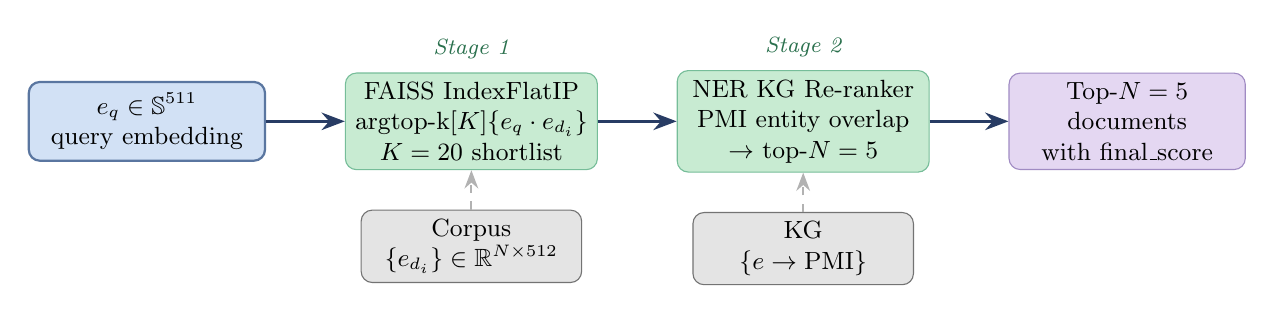
\begin{tikzpicture}[node distance=0.65cm and 1.0cm]
  \node[encnode,minimum width=3.0cm] (qemb) {$e_q \in \Sph^{511}$\\query embedding};
  \node[retnode,right=1.0cm of qemb] (faiss) {FAISS IndexFlatIP\\$\argtopk[K]\{e_q \cdot e_{d_i}\}$\\$K = 20$ shortlist};
  \node[retnode,right=1.0cm of faiss] (kgrank) {NER KG Re-ranker\\PMI entity overlap\\$\to$ top-$N=5$};
  \node[outnode,right=1.0cm of kgrank] (topn) {Top-$N = 5$\\documents\\with final\_score};
  \node[datanode,below=0.5cm of faiss] (corpus) {Corpus\\$\{e_{d_i}\} \in \R^{N \times 512}$};
  \node[datanode,below=0.5cm of kgrank] (kg) {KG\\$\{e \to \text{PMI}\}$};

  \draw[thickarr] (qemb)--(faiss); \draw[thickarr] (faiss)--(kgrank); \draw[thickarr] (kgrank)--(topn);
  \draw[dasharr] (corpus.north)--(faiss.south); \draw[dasharr] (kg.north)--(kgrank.south);
  \node[font=\footnotesize\itshape,color=mintgreen!70!black,above=0.05cm of faiss] {Stage 1};
  \node[font=\footnotesize\itshape,color=mintgreen!70!black,above=0.05cm of kgrank] {Stage 2};
\end{tikzpicture}
\caption{Two-stage hybrid retrieval: dense FAISS search followed by KG PMI re-ranking.}
\label{fig:retrieval}
\end{figure}

\subsection{Stage 1: FAISS Dense Retrieval}

\begin{definition}[FAISS IndexFlatIP]
\[
  \text{dense\_score}(q, d_i) = e_q \cdot e_{d_i} \in [-1,1], \quad
  \mathcal{R}_K = \argtopk_{i}\;(e_q \cdot e_{d_i})
\]
For $N = 69{,}866$ ROCO vectors, exact inner-product search requires $O(N \cdot d) \approx 3.6 \times 10^7$ MACs ($\approx$1\,ms GPU, 15\,ms CPU).
\end{definition}

\subsection{Stage 2: PMI Entity Re-ranking}

\begin{algorithm}[H]
\caption{NER KG Re-ranker (Full Algorithm)}
\label{alg:rerank}
\begin{algorithmic}[1]
\Require Shortlist $S = [d_1,\ldots,d_K]$ with dense\_score; query entities $\mathcal{E}_q$; KG; $\alpha = 0.7$
\Ensure Top-$N$ documents with final\_score $\in [0,1]$
\State $s_{\min} \gets \min_i \text{dense\_score}(d_i)$;\; $s_{\max} \gets \max_i \text{dense\_score}(d_i)$;\; $\Delta \gets \max(s_{\max}-s_{\min}, 10^{-6})$
\State $\tilde{s}_{\text{dense}}(d_i) \gets (\text{dense\_score}(d_i) - s_{\min}) / \Delta$
\ForEach{$d_i \in S$}
  \State $\mathcal{E}_{d_i} \gets \text{word-boundary regex extraction from } d_i.\text{text}$
  \State $\text{kg\_raw}(d_i) \gets \sum_{q \in \mathcal{E}_q}\sum_{d \in \mathcal{E}_{d_i}} \text{PMI}(q,d) \cdot \mathbf{1}[q \in \KG,\; d \in \KG[q]]$
\EndFor
\State $m_{\KG} \gets \max_i \text{kg\_raw}(d_i)$;\quad $\tilde{s}_{\KG}(d_i) \gets \text{kg\_raw}(d_i) / \max(m_{\KG}, 10^{-6})$
\ForEach{$d_i \in S$}
  \State $\text{final\_score}(d_i) \gets \alpha \cdot \tilde{s}_{\text{dense}}(d_i) + (1-\alpha)\cdot\tilde{s}_{\KG}(d_i)$
\EndFor
\State \Return $\text{top-}N(S,\; \text{by final\_score desc})$
\end{algorithmic}
\end{algorithm}

\begin{theorem}[Score Bounds]
$\text{final\_score}(d_i) \in [0,1]$ for all $d_i \in S$ under Algorithm~\ref{alg:rerank}, since $\tilde{s}_{\text{dense}}, \tilde{s}_{\KG} \in [0,1]$ by min-max normalisation and $\alpha + (1-\alpha) = 1$.
\end{theorem}

\subsection{Tiered Confidence and RAG Generation}

\begin{definition}[Confidence Tier Function]
\[
  \text{tier}(s) = \begin{cases}
    \texttt{full}     & s \ge \tau \\
    \texttt{partial}  & \tau - 0.2 \le s < \tau \\
    \texttt{rejected} & s < \tau - 0.2
  \end{cases}, \quad
  \tau_{\text{general}} = 0.40,\; \tau_{\text{medical}} = 0.55.
\]
\end{definition}

\begin{axiom}[Clinical Safety Constraint]
For clinical domains, false positives carry higher risk than false negatives:
$\tau_{\text{medical}} = \tau_{\text{general}} + 0.15$.
\end{axiom}

\begin{algorithm}[H]
\caption{Full Query Pipeline (MIVA-KNIGHT Inference)}
\label{alg:query}
\begin{algorithmic}[1]
\Require user\_input: TextQuery or AudioQuery; loaded pipeline
\Ensure GeneratorOutput: answer, sources, emotion, audio (optional)
\If{user\_input is AudioQuery}
  \State (transcript, emotion, conf\_emo) $\gets$ AudioEncoder.encode$(a)$
  \If{transcript $= \varnothing$} \Return rejection \EndIf
  \State $(e_q, \mathcal{E}_q, h) \gets$ TextEncoder.encode(transcript)
\Else
  \State $(e_q, \mathcal{E}_q, h) \gets$ TextEncoder.encode$(q)$; emotion $\gets$ ``neutral''
\EndIf
\If{$h \ne \varnothing$} \Call{SwapDomain}{MedicalDomain if $h=$``medical'' else GeneralDomain} \EndIf
\State $(\mathcal{D}^*, s_{\max}) \gets$ HybridRetriever.retrieve$(e_q, \mathcal{E}_q)$
\State tier $\gets$ tier$(s_{\max})$
\If{tier $=$ ``rejected''} \Return \textsc{TieredRejection}(domain.name) \EndIf
\State $g \gets$ GeneratorInput$(q, \text{emotion}, \text{conf\_emo}, \mathcal{D}^*, \Pi, \text{tier})$
\State result $\gets$ Generator.generate$(g)$
\If{TTS enabled} result.audio $\gets$ gTTS.convert(result.answer) \EndIf
\State \Return result
\end{algorithmic}
\end{algorithm}

\begin{theorem}[RAG Faithfulness]
An answer is \emph{faithful} to retrieved context $\mathcal{D}^*$ iff every claim $c$ in the answer can be inferred from some $d_j \in \mathcal{D}^*$. MIVA-KNIGHT enforces faithfulness by: (1) ``Answer using ONLY the retrieved context'', (2) requiring citation, (3) rejecting low-confidence retrievals before any LLM call.
\end{theorem}

%%
%% ============================================================
%% PART VIII — PIPELINE C: RAVDESS AUDIO EMOTION
%% ============================================================
%%
\newpage
\section{Pipeline C: RAVDESS Standalone Audio Emotion Recognition}
\label{sec:pipelineC}

\subsection{Design Rationale}

Pipeline~C isolates audio emotion learning from cross-modal interference. Two critical bugs from earlier training are fixed:

\begin{tcolorbox}[keybox,title={Two Bugs Fixed by Pipeline C}]
\textbf{Bug 1 (Contaminated Training):} RAVDESS audio was jointly trained with COCO images under one InfoNCE loss, corrupting the shared space with synthetic negative pairs.\\
\textbf{Bug 2 (Wrong Dimension):} AudioProjection used \texttt{wav2vec\_dim=512} instead of 768, creating a near-identity map with no learning capacity.
\end{tcolorbox}

\begin{axiom}[Standalone Modality Training]
Audio emotion representations must be learned from audio labels alone, without cross-modal entanglement. The only valid supervisory signal for RAVDESS is the emotion label embedded in each filename.
\end{axiom}

\begin{axiom}[Correct Feature Dimensionality]
Wav2Vec 2.0 base outputs $768$-dimensional hidden states. All components must use $d_{\text{in}} = 768$.
\end{axiom}

\subsection{Wav2Vec 2.0 Backbone}

\begin{definition}[Mean-Pool Audio Embedding]
Let $H = [h_1,\ldots,h_{T'}] \in \R^{T' \times 768}$ be Wav2Vec 2.0's last-layer hidden states for a clip of $T \approx 48{,}000$ samples (3\,s at 16\,kHz):
\[
  e_{\text{wav}} = \frac{1}{T'}\sum_{t=1}^{T'} h_t \in \R^{768}, \quad T' \approx 150.
\]
\end{definition}

\begin{figure}[H]
\centering
\begin{adjustbox}{max width=\textwidth}
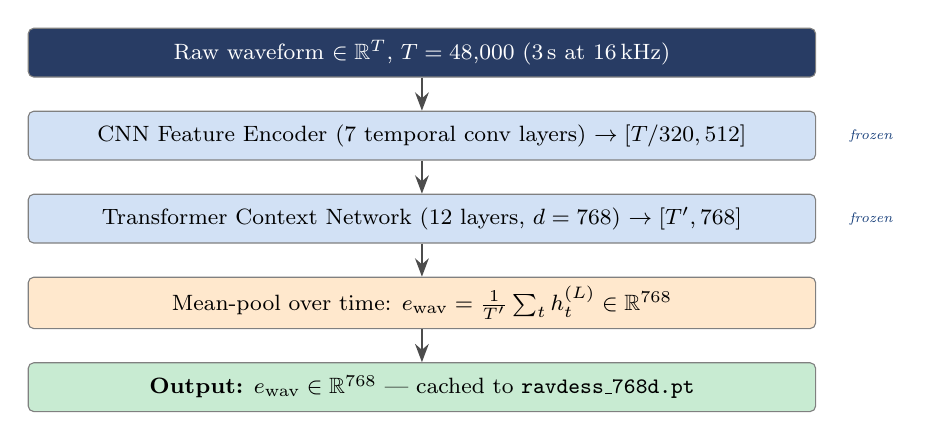
\begin{tikzpicture}[node distance=0.42cm,
  stk/.style={rectangle,rounded corners=2pt,draw=black!50,fill=boxblue,
    align=center,font=\footnotesize,minimum width=10cm,minimum height=0.62cm}]
  \node[stk,fill=cDark,text=white] (inp) {Raw waveform $\in \R^T$, $T = 48{,}000$ (3\,s at 16\,kHz)};
  \node[stk,below=of inp] (cnn) {CNN Feature Encoder (7 temporal conv layers) $\to [T/320, 512]$};
  \node[stk,below=of cnn] (tf) {Transformer Context Network (12 layers, $d=768$) $\to [T', 768]$};
  \node[stk,below=of tf,fill=boxorange] (pool) {Mean-pool over time: $e_{\text{wav}} = \frac{1}{T'}\sum_t h_t^{(L)} \in \R^{768}$};
  \node[stk,below=of pool,fill=boxgreen] (out) {\textbf{Output:} $e_{\text{wav}} \in \R^{768}$ — cached to \texttt{ravdess\_768d.pt}};
  \foreach \a/\b in {inp/cnn,cnn/tf,tf/pool,pool/out} \draw[arr] (\a)--(\b);
  \node[right=0.3cm of cnn,font=\tiny\itshape,color=navyblue] {frozen};
  \node[right=0.3cm of tf,font=\tiny\itshape,color=navyblue] {frozen};
\end{tikzpicture}
\end{adjustbox}
\caption{Wav2Vec 2.0 feature extraction pipeline. All layers frozen during Pipeline~C training.}
\label{fig:wav2vec}
\end{figure}

\begin{lemma}[Caching Speed-up]
Without caching: $T_{\text{no-cache}} = 1{,}440 \times 30 \times 0.3\,\text{s} \approx 3.6\,\text{h}$.
With caching: $T_{\text{cached}} = 120 + 30 \times 0.3 = 129\,\text{s} \approx 2\,\text{min}$.
Speed-up $\approx 100\times$.
\end{lemma}

\begin{algorithm}[H]
\caption{Extract and Cache RAVDESS Embeddings at 768d}
\label{alg:cache_ravdess}
\begin{algorithmic}[1]
\Require RAVDESS\_DIR; CACHE\_768\_FILE
\Ensure dict: filename $\to$ \{embedding $\in \R^{768}$, emotion, actor\_id, intensity\}
\If{CACHE\_768\_FILE exists} load; \textbf{assert} dim $= 768$; \Return cache \EndIf
\For{each Actor\_XX directory (24 actors)}
  \For{each \texttt{.wav} file}
    \State meta $\gets$ \textsc{ParseRavdessFilename}(filename) \Comment{Emotion from field 3}
    \If{meta is None} \textbf{skip} \EndIf
    \State $e \gets$ Wav2VecEncoder.encode(wav\_path).squeeze(0) \quad $\in \R^{768}$
    \State cache[filename] $\gets$ \{embedding: $e$, emotion: meta.emotion, \ldots\}
  \EndFor
\EndFor
\State torch.save(cache, CACHE\_768\_FILE)
\State \textbf{del} encoder; cuda.empty\_cache() \Comment{Free 360\,MB VRAM}
\end{algorithmic}
\end{algorithm}

\subsection{AudioProjection Architecture}

\begin{definition}[AudioProjection $f_\theta$ for Pipeline C]
$f_\theta : \R^{768} \to \Sph^{511}$ is defined by Definition~\ref{def:projmlp} with $d_{\text{in}} = 768$:
\[
  f_\theta(x) = \frac{\LN_{512}(W_2 \cdot \GELU(\LN_{768}(W_1 x + b_1)) + b_2)}
  {\Norm{\LN_{512}(\ldots)}_2}
\]
Total trainable parameters: $768^2 + 768 + 2 \times 768 + 768 \times 512 + 512 + 2 \times 512 = 986{,}880$.
\end{definition}

\subsection{Supervised Contrastive Loss (SupCon)}

The key motivation for SupCon over InfoNCE is:

\begin{center}
\renewcommand{\arraystretch}{1.15}
\begin{tabular}{lll}
\toprule
\textbf{Property} & \textbf{InfoNCE} & \textbf{SupCon} \\
\midrule
Requires & 2 paired modalities & Emotion labels only \\
Positives/anchor & Exactly 1 & All same-class clips in batch \\
Works without text? & No & Yes \\
Multi-class? & No natural support & Designed for $C$ classes \\
\bottomrule
\end{tabular}
\end{center}

\begin{definition}[Supervised Contrastive Loss]
For batch $B$ with labels $\{y_i\}$, positive set $\mathcal{P}(i) = \{p \ne i : y_p = y_i\}$:
\[
  \boxed{\mathcal{L}_{\text{SupCon}} = \frac{1}{B}\sum_{i=1}^B \frac{-1}{|\mathcal{P}(i)|}
  \sum_{p \in \mathcal{P}(i)} \log\frac{\exp(\hat{e}_i \cdot \hat{e}_p / \tau)}{\sum_{a \ne i} \exp(\hat{e}_i \cdot \hat{e}_a / \tau)}}
\]
with $\tau = 0.07$.
\end{definition}

\begin{theorem}[SupCon Random Baseline]
For $B=16$ balanced over $C=8$ classes: $\mathcal{L}_{\text{SupCon}}^{\text{random}} \approx \log(B-1) = \log 15 \approx 2.71$. Target after 30 epochs: $\mathcal{L} < 1.0$.
\end{theorem}

\begin{lemma}[Temperature Effect on Gradient Magnitude]
$\Norm{\partial\mathcal{L}/\partial S_{ij}} \propto 1/\tau$. At $\tau=0.07$, gradients are $\approx 14\times$ larger than at $\tau=1.0$, producing tighter emotion clusters.
\end{lemma}

\begin{algorithm}[H]
\caption{SupCon Loss Computation}
\label{alg:supcon_c}
\begin{algorithmic}[1]
\Require Embeddings $E \in \R^{B \times D}$; labels $y \in \mathbb{Z}^B$; temperature $\tau$
\Ensure Scalar loss
\State $\hat{E} \gets E / \Norm{E}_2$ (row-wise L2-normalise)
\State $\text{sim} \gets \hat{E}\hat{E}^\top / \tau$ \quad $[B,B]$
\State pos\_mask$[i,j] \gets \mathbf{1}[y_i = y_j \wedge i \ne j]$
\State $\text{sim} \gets \text{sim} - \max(\text{sim}, \text{dim=1})$ \Comment{Log-sum-exp stability}
\State $\text{exp\_sim} \gets \exp(\text{sim}) \odot (1 - I_B)$ \Comment{Exclude self}
\State $\text{log\_prob} \gets \text{sim} - \log(\text{exp\_sim.sum(dim=1)} + \varepsilon)$
\State $n_{\text{pos}} \gets \text{pos\_mask.sum(dim=1)}$; valid $\gets (n_{\text{pos}} > 0)$
\If{valid.sum() $= 0$} \Return 0 \EndIf
\State per\_anchor $\gets -(\text{pos\_mask} \odot \text{log\_prob}).\text{sum(dim=1)}$
\State \Return mean(per\_anchor[valid] / $n_{\text{pos}}$[valid])
\end{algorithmic}
\end{algorithm}

\subsection{Training Loop and Centroid Evaluation}

\begin{algorithm}[H]
\caption{Pipeline C Single Training Epoch (SupCon)}
\label{alg:supcon_epoch}
\begin{algorithmic}[1]
\Require audio\_loader; audio\_proj $f_\theta$; optimizer; scheduler
\Ensure Mean epoch SupCon loss
\State audio\_proj.train()
\ForEach{$(E_b \in \R^{B \times 768},\; y_b \in \mathbb{Z}^B)$ in audio\_loader}
  \State $\hat{E} \gets f_\theta(E_b.\text{to(device)})$ \quad $[B, 512]$ on $\Sph^{511}$
  \State $\ell \gets \mathcal{L}_{\text{SupCon}}(\hat{E}, y_b, \tau{=}0.07)$
  \State optimizer.zero\_grad(); $\ell$.backward()
  \State clip\_grad\_norm$(f_\theta.\text{parameters}(), c=1.0)$
  \State optimizer.step(); scheduler.step()
\EndFor
\end{algorithmic}
\end{algorithm}

\begin{definition}[Spherical Centroid]
For emotion class $e$ with $N_e$ projected embeddings $\{\hat{a}_i^{(e)}\} \subset \Sph^{511}$:
\[
  \bar{c}_e = \frac{\mu_e}{\Norm{\mu_e}_2}, \quad \mu_e = \frac{1}{N_e}\sum_{i=1}^{N_e}\hat{a}_i^{(e)}.
\]
\end{definition}

\begin{lemma}[Centroid Optimality on $\Sph^{511}$]
The spherical centroid $\bar{c}_e$ minimises $\sum_{i=1}^{N_e} \arccos^2(\hat{a}_i^{(e)} \cdot v)$ over $v \in \Sph^{511}$.
\end{lemma}

\begin{algorithm}[H]
\caption{Emotion Accuracy Evaluation via Centroid Nearest-Neighbour}
\label{alg:centroid_eval}
\begin{algorithmic}[1]
\Require audio\_proj $f_\theta$; data loader
\Ensure overall accuracy; per-emotion dict; centroids $[C, 512]$
\State audio\_proj.eval()
\State $E \gets \text{cat}([f_\theta(E_b) \text{ for each batch}])$ \quad $[N, 512]$
\State $Y \gets \text{cat}([y_b \text{ for each batch}])$ \quad $[N]$
\For{$c = 0$ to $C-1$}
  \State $\bar{c}_c \gets \text{L2-norm}(E[Y{=}c].\text{mean(dim=0)})$
\EndFor
\State $C_{\text{mat}} \gets \text{stack}(\bar{c}_0,\ldots,\bar{c}_{C-1})$ \quad $[C, 512]$
\State predicted $\gets \argmax(E \cdot C_{\text{mat}}^\top, \text{dim=1})$
\State accuracy $\gets \text{mean}(\text{predicted} = Y)$
\State \Return accuracy, per-emotion breakdown, $C_{\text{mat}}$
\end{algorithmic}
\end{algorithm}

\begin{tcolorbox}[laymanbox]
SupCon is a team-building exercise. Each audio clip looks at all other clips in the batch. Same-emotion clips (teammates) are pulled closer; different-emotion clips are pushed apart. Temperature $\tau = 0.07$ makes the criterion very strict — only genuinely similar teammates score well.
\end{tcolorbox}

%%
%% ============================================================
%% PART IX — PIPELINE D: CREMA-D AUDIO-VISUAL EMOTION
%% ============================================================
%%
\newpage
\section{Pipeline D: CREMA-D Audio-Visual Emotion Recognition}
\label{sec:pipelineD}

\subsection{Overview and Three-Phase Training Strategy}

Pipeline~D extends emotion recognition to the CREMA-D dataset (7,442 clips, 91 actors, 6 emotions) using \emph{two frozen backbones}: Wav2Vec 2.0 (94M, audio) and ResNet-50 (23M, middle frame video). Only projection heads ($\approx$3.6M params) train.

\begin{table}[H]
\centering
\caption{Three-phase Pipeline D training history}
\begin{tabularx}{\textwidth}{lXXXXX}
\toprule
& \textbf{Notebook} & \textbf{Loss} & \textbf{LR} & \textbf{Epochs} & \textbf{Result} \\
\midrule
Phase 1 & Pipeline D v3 & Cross-modal InfoNCE & $10^{-4}$ & 13 & 42.2\% (1/6) \\
Phase 2 & Pipeline D v3 & SupCon & $10^{-5}$ & 10 & 43.9\% (3/6) \\
Phase 3 & Phase 3 nb & \textbf{SupCon} & $\mathbf{5\times10^{-5}}$ & \textbf{15} & \textbf{Target $\geq$ 4/6} \\
\bottomrule
\end{tabularx}
\end{table}

\begin{figure}[H]
\centering
\begin{adjustbox}{max width=\textwidth}
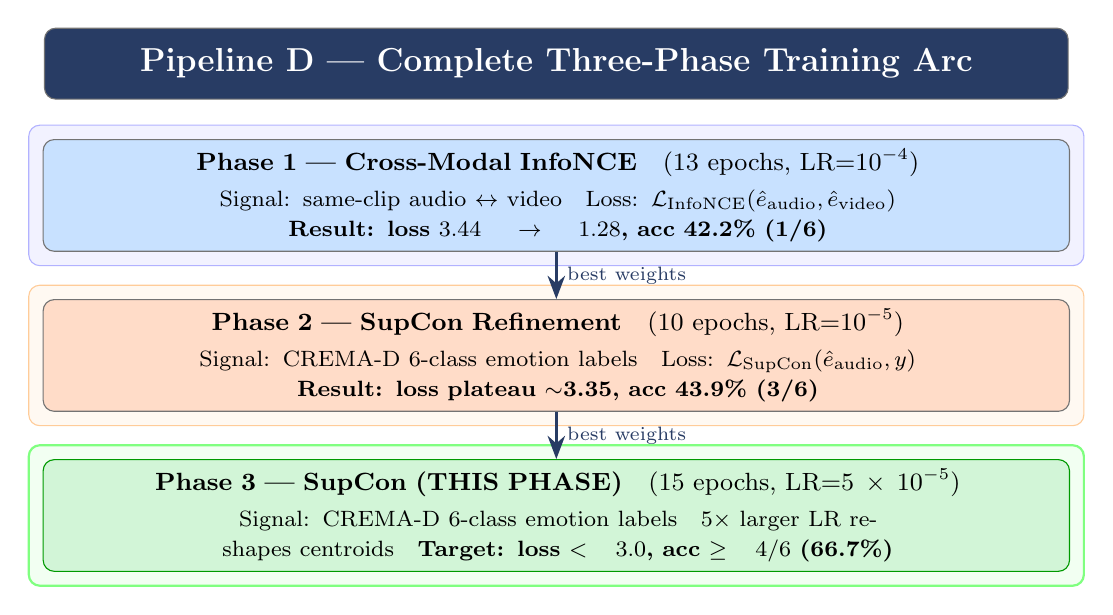
\begin{tikzpicture}[node distance=0.7cm]
  \node[basebox,fill=cDark,text=white,minimum width=13cm,minimum height=0.9cm] (hdr)
      {\large\bfseries Pipeline D — Complete Three-Phase Training Arc};
  \node[basebox,fill=cPhase1,minimum width=13cm,minimum height=1.3cm,text width=12.8cm,
        below=0.5cm of hdr] (p1)
      {\textbf{Phase 1 — Cross-Modal InfoNCE}\quad(13 epochs, LR=$10^{-4}$)\\[2pt]
       \footnotesize Signal: same-clip audio $\leftrightarrow$ video\quad
       Loss: $\mathcal{L}_{\text{InfoNCE}}(\hat{e}_{\text{audio}}, \hat{e}_{\text{video}})$\quad
       \textbf{Result: loss $3.44\to1.28$, acc 42.2\% (1/6)}};
  \node[basebox,fill=cPhase2,minimum width=13cm,minimum height=1.3cm,text width=12.8cm,
        below=0.6cm of p1] (p2)
      {\textbf{Phase 2 — SupCon Refinement}\quad(10 epochs, LR=$10^{-5}$)\\[2pt]
       \footnotesize Signal: CREMA-D 6-class emotion labels\quad
       Loss: $\mathcal{L}_{\text{SupCon}}(\hat{e}_{\text{audio}}, y)$\quad
       \textbf{Result: loss plateau $\sim$3.35, acc 43.9\% (3/6)}};
  \node[basebox,fill=cPhase3,draw=green!60!black,minimum width=13cm,minimum height=1.3cm,
        text width=12.8cm,below=0.6cm of p2] (p3)
      {\textbf{Phase 3 — SupCon (THIS PHASE)}\quad(15 epochs, LR=$5\times10^{-5}$)\\[2pt]
       \footnotesize Signal: CREMA-D 6-class emotion labels\quad
       5$\times$ larger LR reshapes centroids\quad
       \textbf{Target: loss $< 3.0$, acc $\geq 4/6$ (66.7\%)}};

  \draw[thickarr] (p1.south) -- (p2.north) node[midway,right,font=\scriptsize]{best weights};
  \draw[thickarr] (p2.south) -- (p3.north) node[midway,right,font=\scriptsize]{best weights};

  \begin{pgfonlayer}{background}
    \node[rectangle,draw=blue!30,fill=blue!5,rounded corners,fit=(p1),inner sep=5pt] {};
    \node[rectangle,draw=orange!40,fill=orange!5,rounded corners,fit=(p2),inner sep=5pt] {};
    \node[rectangle,draw=green!50,fill=green!5,thick,rounded corners,fit=(p3),inner sep=5pt] {};
  \end{pgfonlayer}
\end{tikzpicture}
\end{adjustbox}
\caption{Pipeline D three-phase training arc: InfoNCE alignment $\to$ SupCon cluster sharpening $\to$ higher-LR SupCon refinement.}
\label{fig:pipeline_d_phases}
\end{figure}

\subsection{VideoFrameProjection Architecture}

\begin{definition}[VideoFrameProjection $f_\phi^{\text{video}}$]
Let $I \in \R^{3 \times 224 \times 224}$ be an ImageNet-normalised middle frame.
\[
  f_\phi^{\text{video}}(I) = \text{L2-norm}\!\left(\LN_{512}(W_4 \cdot \GELU(\LN_{1024}(W_3 \cdot r(I) + b_3)) + b_4)\right)
\]
where $r(I) = \text{ResNet50}(I) \in \R^{2048}$ (frozen), $W_3 \in \R^{1024 \times 2048}$, $W_4 \in \R^{512 \times 1024}$. Trainable: $\approx$2.63\,M parameters.
\end{definition}

\begin{algorithm}[H]
\caption{CREMA-D Middle-Frame Extraction}
\label{alg:frame_extract}
\begin{algorithmic}[1]
\Require mp4\_path; FRAME\_TRANSFORM (Resize224$\to$CentCrop$\to$ToTensor$\to$ImageNetNorm)
\Ensure $(f, \text{success})$, $f \in \R^{3 \times 224 \times 224}$
\State cap $\gets$ cv2.VideoCapture(mp4\_path)
\If{not cap.isOpened()} \Return (GrayFallback, False) \EndIf
\State $N \gets$ cap.get(CAP\_PROP\_FRAME\_COUNT)
\State cap.set(CAP\_PROP\_POS\_FRAMES, $\max(0, \lfloor N/2 \rfloor)$) \Comment{Seek to midpoint}
\State (ret, frame) $\gets$ cap.read(); cap.release()
\If{not ret} \Return (GrayFallback, False) \EndIf
\State rgb $\gets$ cv2.cvtColor(frame, COLOR\_BGR2RGB)
\State $f \gets$ FRAME\_TRANSFORM(Image.fromarray(rgb))
\State \Return $(f, \text{True})$
\end{algorithmic}
\end{algorithm}

\begin{theorem}[Peak Expression Frame]
The middle frame of a short acted-emotion clip ($\le 3$\,s) maximises the probability of capturing the peak facial action unit configuration, as actors complete their ramp-up in the first half and relax in the final quarter.
\end{theorem}

\subsection{Cross-Modal InfoNCE (Stage 1)}

\begin{definition}[Cross-Modal InfoNCE Loss for Pipeline D]
For $B$ audio-video pairs with $S_{ij} = \hat{e}_i^{\text{audio}} \cdot \hat{e}_j^{\text{video}}$:
\[
  \mathcal{L}_{\text{InfoNCE}} = \frac{1}{2}\!\left[
    -\frac{1}{B}\sum_i \log\frac{e^{S_{ii}/\tau}}{\sum_j e^{S_{ij}/\tau}}
    -\frac{1}{B}\sum_j \log\frac{e^{S_{jj}/\tau}}{\sum_i e^{S_{ij}/\tau}}
  \right]
\]
Random baseline: $\mathcal{L}^{\text{random}} = \log B = \log 32 \approx 3.47$.
\end{definition}

\begin{theorem}[InfoNCE Lower Bound on Mutual Information]
Maximising $-\mathcal{L}_{\text{InfoNCE}}$ is equivalent to maximising a lower bound:
$I(A; V) \ge \log B - \mathcal{L}_{\text{InfoNCE}}$.
\end{theorem}

\begin{algorithm}[H]
\caption{Stage 1: Full Cross-Modal InfoNCE Training (13 epochs)}
\label{alg:stage1_d}
\begin{algorithmic}[1]
\Require audio\_proj (warm-start from Pipeline~C); video\_proj (random init); $E = 13$
\For{$e = 0$ to $E-1$}
  \ForEach{$(e_{\text{wav}}^{[B,768]}, \text{frame}^{[B,3,224,224]}, \text{labels}^{[B]})$ in loader}
    \State $\hat{e}_A \gets \text{audio\_proj}(e_{\text{wav}}.\text{to(device)})$ \quad $[B,512]$
    \State $\hat{e}_V \gets \text{video\_proj}(\text{frame}.\text{to(device)})$ \quad (ResNet inside no\_grad)
    \State $\mathcal{L} \gets \mathcal{L}_{\text{InfoNCE}}(\hat{e}_A, \hat{e}_V, \tau{=}0.07)$
    \State optimizer.zero\_grad(); $\mathcal{L}$.backward()
    \State ClipGradNorm(params, $c = 1.0$)
    \State optimizer.step(); scheduler.step()
  \EndFor
  \State acc $\gets$ \textsc{EvaluateAccuracy}()
  \If{acc $>$ best\_acc} save best\_audio\_sd, best\_video\_sd \EndIf
  \State \textsc{SaveCheckpoint}($e$)
\EndFor
\end{algorithmic}
\end{algorithm}

\subsection{Stage 2 and Phase 3: SupCon Refinement}

\begin{theorem}[Phase 2 LR Insufficiency]
Phase 2's LR $= 10^{-5}$ was insufficient to meaningfully reposition centroids. Weight update per step:
$\Delta_{\text{Phase 2}} \approx 10^{-5} \times 12.4 \approx 1.24 \times 10^{-4}$ (marginal). Phase~3: $\Delta_{\text{Phase 3}} \approx 5 \times 10^{-5} \times 12.4 \approx 6.2 \times 10^{-4}$ (meaningful, while preserving InfoNCE geometry).
\end{theorem}

\begin{theorem}[Transfer Learning Benefit (Warm-Start)]
Pipeline~D AudioProjection inherits Pipeline~C (RAVDESS) weights. Since RAVDESS and CREMA-D share 6/8 emotion classes (\textit{angry, disgust, fearful, happy, neutral, sad}), inherited weights provide useful initial geometry, reducing InfoNCE epochs needed.
\end{theorem}

\begin{lemma}[Geometry Preservation Under Low LR (Stage 2)]
For small perturbations $\delta\theta$ to InfoNCE-trained weights $\theta^*$: $f_{\theta^*+\delta\theta}(x) \approx f_{\theta^*}(x) + J_\theta \delta\theta$. With $\eta_2 = 10^{-5}$, $\|\delta\theta\| \approx 3 \times 10^{-6}$ per step — small enough to preserve cross-modal InfoNCE geometry while tightening class boundaries.
\end{lemma}

\begin{lemma}[SupCon Cluster Geometry]
Under SupCon minimisation, the optimal geometry concentrates class $c$ at $\bar{c}_c = \mu_c/\Norm{\mu_c}$, with inter-class angle approaching $\theta_{cc'} = \arccos(-1/(K-1))$, $K=6$ — the maximum-separation packing (regular simplex inscribed in $\Sph^{511}$).
\end{lemma}

%%
%% ============================================================
%% PART X — PIPELINE E: CMU-MOSI SENTIMENT FUSION
%% ============================================================
%%
\newpage
\section{Pipeline E: CMU-MOSI Multimodal Sentiment Fusion}
\label{sec:pipelineE}

\subsection{Overview}

Pipeline~E processes three concurrent data streams from the CMU-MOSI corpus (2,199 video opinion segments, 93 YouTube videos, sentiment $y \in [-3, +3]$) using a cross-modal Transformer encoder. This is the fullest realisation of the model-based multimodal fusion taxonomy cell.

\begin{figure}[H]
\centering
\resizebox{\textwidth}{!}{%
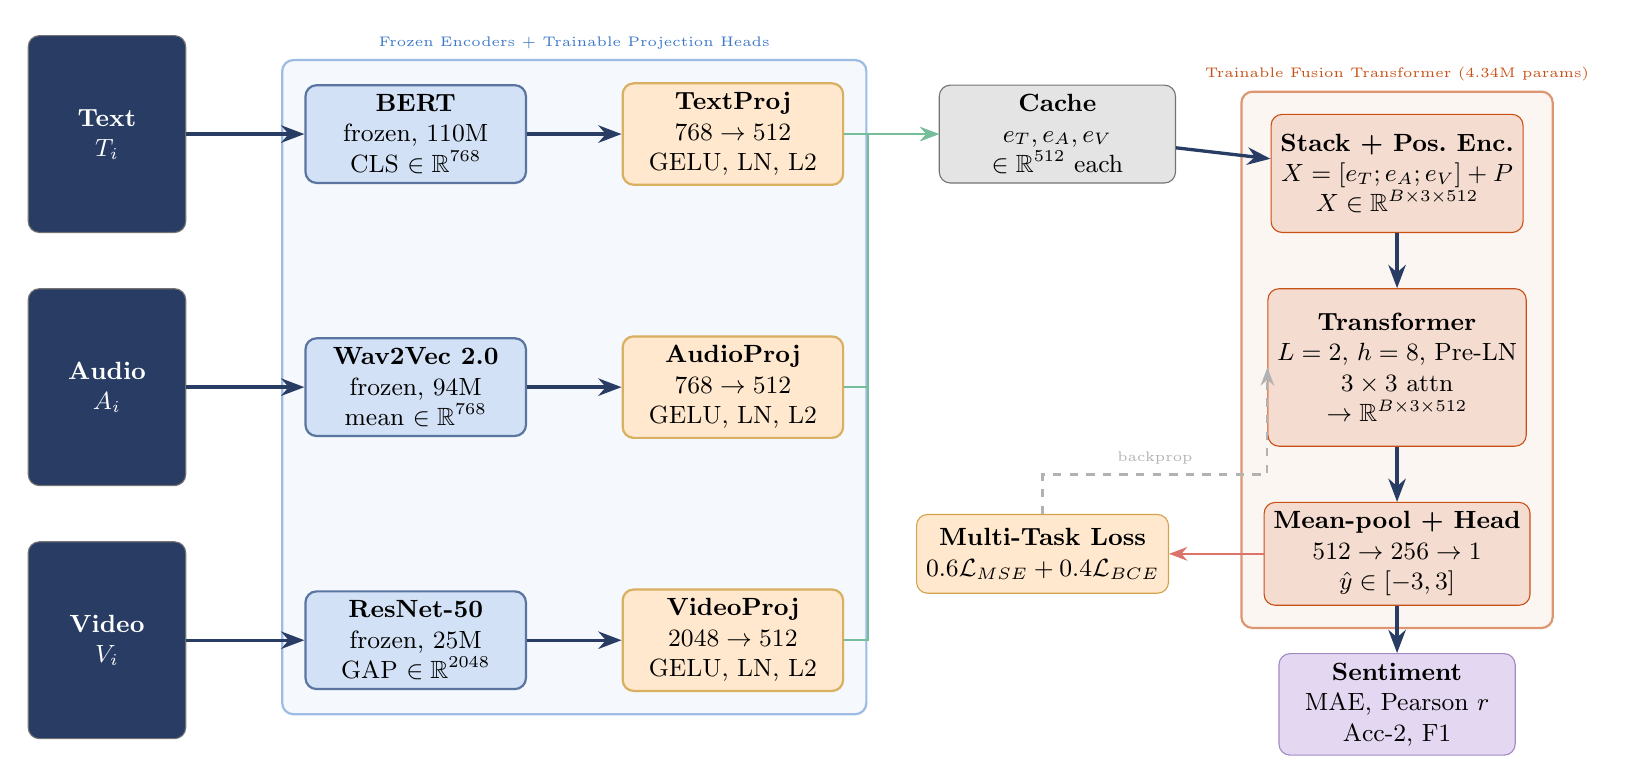
\begin{tikzpicture}[node distance=1.0cm and 1.3cm]
  \node[inputnode,minimum width=2.0cm,minimum height=2.5cm] (textIn) at (0,0) {\textbf{Text}\\$T_i$};
  \node[inputnode,minimum width=2.0cm,minimum height=2.5cm,below=0.7cm of textIn] (audioIn) {\textbf{Audio}\\$A_i$};
  \node[inputnode,minimum width=2.0cm,minimum height=2.5cm,below=0.7cm of audioIn] (videoIn) {\textbf{Video}\\$V_i$};

  \node[encnode,right=1.5cm of textIn,minimum width=2.8cm] (bert2) {\textbf{BERT}\\frozen, 110M\\CLS $\in \R^{768}$};
  \node[encnode,right=1.5cm of audioIn,minimum width=2.8cm] (wav2) {\textbf{Wav2Vec 2.0}\\frozen, 94M\\mean $\in \R^{768}$};
  \node[encnode,right=1.5cm of videoIn,minimum width=2.8cm] (res2) {\textbf{ResNet-50}\\frozen, 25M\\GAP $\in \R^{2048}$};

  \node[projnode,right=1.2cm of bert2,minimum width=2.8cm] (tp) {\textbf{TextProj}\\$768\to512$\\GELU, LN, L2};
  \node[projnode,right=1.2cm of wav2,minimum width=2.8cm] (ap) {\textbf{AudioProj}\\$768\to512$\\GELU, LN, L2};
  \node[projnode,right=1.2cm of res2,minimum width=2.8cm] (vp) {\textbf{VideoProj}\\$2048\to512$\\GELU, LN, L2};

  \node[datanode,right=1.2cm of tp,minimum width=3.0cm] (cache) {\textbf{Cache}\\$e_T, e_A, e_V$\\$\in \R^{512}$ each};

  \node[basebox,fill=fusioncolor!20,draw=fusioncolor,minimum width=3.2cm,minimum height=1.5cm,
        right=1.2cm of cache,yshift=-0.5cm] (stack)
      {\textbf{Stack + Pos.\ Enc.}\\$X = [e_T;e_A;e_V]+P$\\$X \in \R^{B \times 3 \times 512}$};

  \node[basebox,fill=fusioncolor!20,draw=fusioncolor,minimum width=3.2cm,minimum height=2.0cm,
        below=0.7cm of stack] (transf)
      {\textbf{Transformer}\\$L=2$, $h=8$, Pre-LN\\$3\times3$ attn\\$\to \R^{B\times3\times512}$};

  \node[basebox,fill=fusioncolor!20,draw=fusioncolor,minimum width=3.2cm,
        below=0.7cm of transf] (reg)
      {\textbf{Mean-pool + Head}\\$512\to256\to1$\\$\hat{y} \in [-3,3]$};

  \node[lossnode,left=1.2cm of reg] (loss2) {\textbf{Multi-Task Loss}\\$0.6\mathcal{L}_{MSE}+0.4\mathcal{L}_{BCE}$};
  \node[outnode,below=0.6cm of reg] (out2) {\textbf{Sentiment}\\MAE, Pearson $r$\\Acc-2, F1};

  \draw[thickarr] (textIn)--(bert2); \draw[thickarr] (audioIn)--(wav2); \draw[thickarr] (videoIn)--(res2);
  \draw[thickarr] (bert2)--(tp); \draw[thickarr] (wav2)--(ap); \draw[thickarr] (res2)--(vp);
  \draw[greenarr] (tp.east) -- ++(0.3,0) |- (cache.west);
  \draw[greenarr] (ap.east) -- ++(0.3,0) |- (cache.west);
  \draw[greenarr] (vp.east) -- ++(0.3,0) |- (cache.west);
  \draw[thickarr] (cache)--(stack);
  \draw[thickarr] (stack)--(transf);
  \draw[thickarr] (transf)--(reg);
  \draw[redarr] (reg)--(loss2);
  \draw[dasharr] (loss2.north) -- ++(0,0.5) -| (transf.west) node[near start,above,font=\tiny]{backprop};
  \draw[thickarr] (reg)--(out2);

  \begin{pgfonlayer}{background}
    \node[rectangle,draw=encodercolor!50,fill=encodercolor!5,thick,rounded corners,
          fit=(bert2)(wav2)(res2)(tp)(ap)(vp),inner sep=8pt,
          label={[font=\tiny,color=encodercolor]above:Frozen Encoders + Trainable Projection Heads}] {};
    \node[rectangle,draw=fusioncolor!60,fill=fusioncolor!5,thick,rounded corners,
          fit=(stack)(transf)(reg),inner sep=8pt,
          label={[font=\tiny,color=fusioncolor]above:Trainable Fusion Transformer (4.34M params)}] {};
  \end{pgfonlayer}
\end{tikzpicture}
}
\caption{Pipeline~E: three-modality fusion for CMU-MOSI sentiment analysis using a cross-modal Transformer.}
\label{fig:pipeline_e}
\end{figure}

\subsection{Multi-Modal Transformer Architecture}

\begin{definition}[MultimodalFusionTransformer]
$\pi_\theta : \R^{512} \times \R^{512} \times \R^{512} \to \R$ consists of:
(1) learnable positional encodings $P \in \R^{3 \times 512}$; (2) $L=2$-layer Pre-LN Transformer with $h=8$ attention heads, $d_{ff}=1024$; (3) mean-pool over 3 tokens; (4) regression head: Linear$(512\!\to\!256)\to\GELU\to\text{Dropout}(0.1)\to$Linear$(256\!\to\!1)$.
\end{definition}

\begin{theorem}[Scaled Dot-Product Attention]
$\text{Attn}(Q,K,V) = \softmax\!\left(\frac{QK^\top}{\sqrt{d_k}}\right)V$. The $1/\sqrt{d_k}$ factor prevents dot products from growing large and pushing softmax to saturation.
\end{theorem}

\begin{theorem}[Multi-Head Attention]
$\MHA(Q,K,V) = \text{Concat}(\text{head}_1,\ldots,\text{head}_h)W^O$. Different heads specialise in distinct cross-modal relationships (e.g., audio-text, video-text alignment).
\end{theorem}

\begin{axiom}[Pre-LN Stability]
Pre-LN architecture: $x' = x + \text{Attn}(\LN(x))$, $x'' = x' + \text{FFN}(\LN(x'))$. Provides more stable gradients during early training compared to Post-LN, because the residual pathway preserves gradient magnitude.
\end{axiom}

\begin{algorithm}[H]
\caption{MultimodalFusionTransformer.forward}
\label{alg:fusion_forward}
\begin{algorithmic}[1]
\Require $\hat{e}_T, \hat{e}_A, \hat{e}_V \in \R^{B \times 512}$; parameters $\theta$
\Ensure Sentiment scores $\hat{y} \in \R^B$
\State $X \gets \text{stack}([\hat{e}_T, \hat{e}_A, \hat{e}_V], \text{dim}=1) \in \R^{B \times 3 \times 512}$
\State $X \gets X + P$ \Comment{Learnable modality positional encodings}
\For{$\ell = 1$ to $L=2$}
  \State $X \gets X + \MHA(\LN(X))$ \Comment{Pre-LN self-attention}
  \State $X \gets X + \text{FFN}(\LN(X))$ \Comment{Pre-LN feed-forward}
\EndFor
\State $\bar{x} \gets X.\text{mean(dim=1)} \in \R^{B \times 512}$
\State $z \gets \GELU(W_1 \bar{x} + b_1) \in \R^{B \times 256}$
\State $z \gets \text{Dropout}(z, p=0.1)$
\State $\hat{y} \gets W_2 z + b_2 \in \R^B$
\State \Return $\hat{y}$
\end{algorithmic}
\end{algorithm}

\subsection{Multi-Task Sentiment Loss}

\begin{definition}[Multi-Task Sentiment Loss]
\[
  \mathcal{L}(\hat{y}, y, b) = 0.6 \cdot \mathcal{L}_{\text{MSE}}(\hat{y}, y) + 0.4 \cdot \mathcal{L}_{\text{BCE}}(\hat{y}, b)
\]
\[
  \mathcal{L}_{\text{MSE}} = \frac{1}{B}\sum_{i=1}^B (\hat{y}_i - y_i)^2, \quad
  \mathcal{L}_{\text{BCE}} = -\frac{1}{B}\sum_{i=1}^B [b_i \log\sigma(\hat{y}_i) + (1-b_i)\log(1-\sigma(\hat{y}_i))]
\]
\end{definition}

\begin{theorem}[Numerical Stability of Logit BCE]
The numerically stable form: $\mathcal{L}_{\text{BCE}}(\hat{y},b) = \max(0,\hat{y}) - b\hat{y} + \log(1 + e^{-|\hat{y}|})$. Avoids overflow/underflow in $e^{\hat{y}}$.
\end{theorem}

\begin{lemma}[L2 Normalisation Maps to Unit Hypersphere]
After L2-normalisation, $\hat{e} = e/\Norm{e}_2$, all embeddings satisfy $\Norm{\hat{e}}_2 = 1$, so $\hat{e}_i^\top \hat{e}_j = \cos(\theta_{ij})$, enabling scale-invariant comparison across modalities.
\end{lemma}

\begin{algorithm}[H]
\caption{Full Training Loop — Pipeline E (20 Epochs, Best-Model Tracking)}
\label{alg:training_e}
\begin{algorithmic}[1]
\Require Model $\pi_\theta$; train/valid loaders; AdamW optimizer; cosine warmup scheduler; $E=20$
\Ensure Best model state $\theta^*$
\State best\_mae $\gets \infty$; $\theta^* \gets$ None
\For{$e = 0$ to $E-1$}
  \ForEach{batch $(T, A, V, y, b)$ in train\_loader}
    \State $\hat{y} \gets \pi_\theta(T, A, V)$
    \State $\mathcal{L} \gets 0.6\mathcal{L}_{\text{MSE}}(\hat{y},y) + 0.4\mathcal{L}_{\text{BCE}}(\hat{y},b)$
    \State optimizer.zero\_grad(); $\mathcal{L}$.backward()
    \State clip\_grad\_norm$(\theta, c=1.0)$; optimizer.step(); scheduler.step()
  \EndFor
  \State MAE$_\text{val} \gets$ Evaluate(valid\_loader)
  \If{MAE$_\text{val} < $ best\_mae}
    \State best\_mae $\gets$ MAE$_\text{val}$; $\theta^* \gets \pi_\theta.\text{state\_dict().clone()}$
  \EndIf
  \State torch.save(checkpoint, path)
\EndFor
\State \Return $\theta^*$ \Comment{Best: epoch 17, val MAE $= 0.7238$}
\end{algorithmic}
\end{algorithm}

\begin{definition}[CMU-MOSI Evaluation Suite]
\textbf{MAE:} $\frac{1}{N}\sum|\hat{y}_i - y_i|$\quad
\textbf{Pearson $r$:} $\frac{\sum(\hat{y}_i-\bar{\hat{y}})(y_i-\bar{y})}{\sqrt{\sum(\hat{y}_i-\bar{\hat{y}})^2\sum(y_i-\bar{y})^2}}$\quad
\textbf{Acc-2:} $\frac{1}{N}\sum\mathbf{1}[\text{sign}(\hat{y}_i)=\text{sign}(y_i)]$\quad
\textbf{Wtd F1:} $\sum_c \frac{n_c}{N}\frac{2P_cR_c}{P_c+R_c}$
\end{definition}

%%
%% ============================================================
%% PART XI — OPTIMISATION
%% ============================================================
%%
\newpage
\section{Optimisation: AdamW and Cosine Scheduling}
\label{sec:optim}

\begin{definition}[AdamW Update Rule]
At step $t$ with gradient $g_t = \nabla_\theta \mathcal{L}_t$:
\[
  m_t = \beta_1 m_{t-1} + (1-\beta_1)g_t, \quad v_t = \beta_2 v_{t-1} + (1-\beta_2)g_t^2
\]
\[
  \hat{m}_t = \frac{m_t}{1-\beta_1^t}, \quad \hat{v}_t = \frac{v_t}{1-\beta_2^t}
\]
\[
  \boxed{\theta_{t+1} = \theta_t - \eta \cdot \frac{\hat{m}_t}{\sqrt{\hat{v}_t}+\varepsilon} - \eta\lambda\theta_t}
\]
$\eta = 10^{-4}$, $\lambda = 0.01$, $\beta_1 = 0.9$, $\beta_2 = 0.999$, $\varepsilon = 10^{-8}$.
\end{definition}

\begin{remark}[Decoupled Weight Decay]
Standard Adam applies weight decay inside the adaptive scaling (incorrect). AdamW applies $\eta\lambda\theta_t$ directly to parameters, giving correct $\ell_2$ regularisation regardless of gradient magnitude.
\end{remark}

\begin{lemma}[Why AdamW over Adam]
Adam with L2 regularisation adds $\lambda\theta$ to the gradient before adaptive scaling, dividing weight decay by $\sqrt{\hat{v}_t}$ and diminishing regularisation for high-variance parameters. AdamW avoids this by applying weight decay after the adaptive step.
\end{lemma}

\begin{definition}[Warmup-Cosine LR Schedule]
Let $T_{\text{total}}$ be total steps, $T_w = T_{\text{total}}/10$ warmup steps:
\[
  \eta(t) = \begin{cases}
    \eta_0 \cdot \dfrac{t}{T_w} & t < T_w \quad\text{(linear warmup)}\\[6pt]
    \dfrac{\eta_0}{2}\!\left(1+\cos\dfrac{\pi(t-T_w)}{T_{\text{total}}-T_w}\right) & t \ge T_w \quad\text{(cosine decay)}
  \end{cases}
\]
\end{definition}

\begin{figure}[H]
\centering
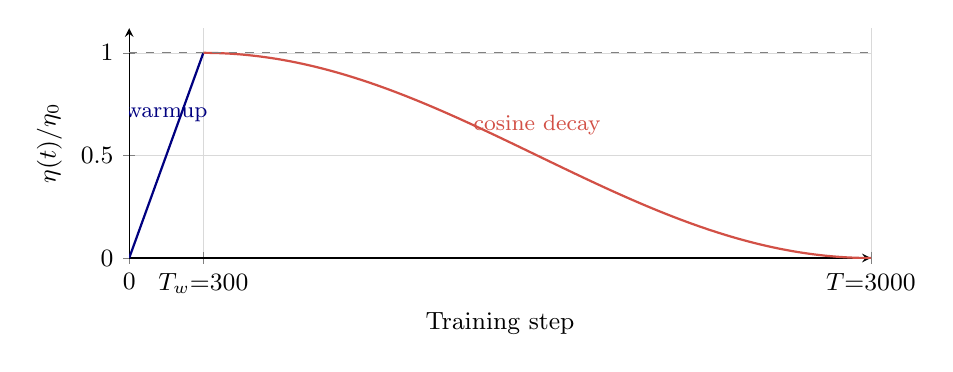
\begin{tikzpicture}
\begin{axis}[
  width=11cm, height=4.5cm,
  xlabel={Training step},
  ylabel={$\eta(t)/\eta_0$},
  xmin=0, xmax=3000, ymin=0, ymax=1.12,
  xtick={0,300,3000},
  xticklabels={0,$T_w{=}300$,$T{=}3000$},
  ytick={0,0.5,1},
  grid=both, grid style={line width=0.2pt,draw=gray!30},
  axis lines=left,
  tick label style={font=\small},
  label style={font=\small}
]
\addplot[NavyBlue,thick,domain=0:300,samples=60] {x/300};
\addplot[coralred,thick,domain=300:3000,samples=200]
  {0.5*(1+cos(deg((x-300)/(3000-300)*pi)))};
\addplot[dashed,gray,domain=0:3000] {1.0};
\node[font=\footnotesize,color=NavyBlue] at (axis cs:150,0.7) {warmup};
\node[font=\footnotesize,color=coralred] at (axis cs:1650,0.65) {cosine decay};
\end{axis}
\end{tikzpicture}
\caption{Warmup-cosine learning rate schedule. Linear warmup for first 10\% of steps; cosine decay thereafter.}
\label{fig:lr_schedule}
\end{figure}

\begin{definition}[Gradient Clipping]
$\tilde{\nabla}_\theta = \min\!\left(1, \frac{c}{\Norm{\nabla_\theta}_2}\right)\nabla_\theta,\; c = 1.0$. Caps the $\ell_2$-norm of all trainable gradients, preventing exploding gradients while preserving direction.
\end{definition}

%%
%% ============================================================
%% PART XII — FULL SYSTEM PIPELINE
%% ============================================================
%%
\newpage
\section{Full MIVA-KNIGHT System Pipeline}
\label{sec:system}

\begin{figure}[H]
\centering
\resizebox{\textwidth}{!}{%
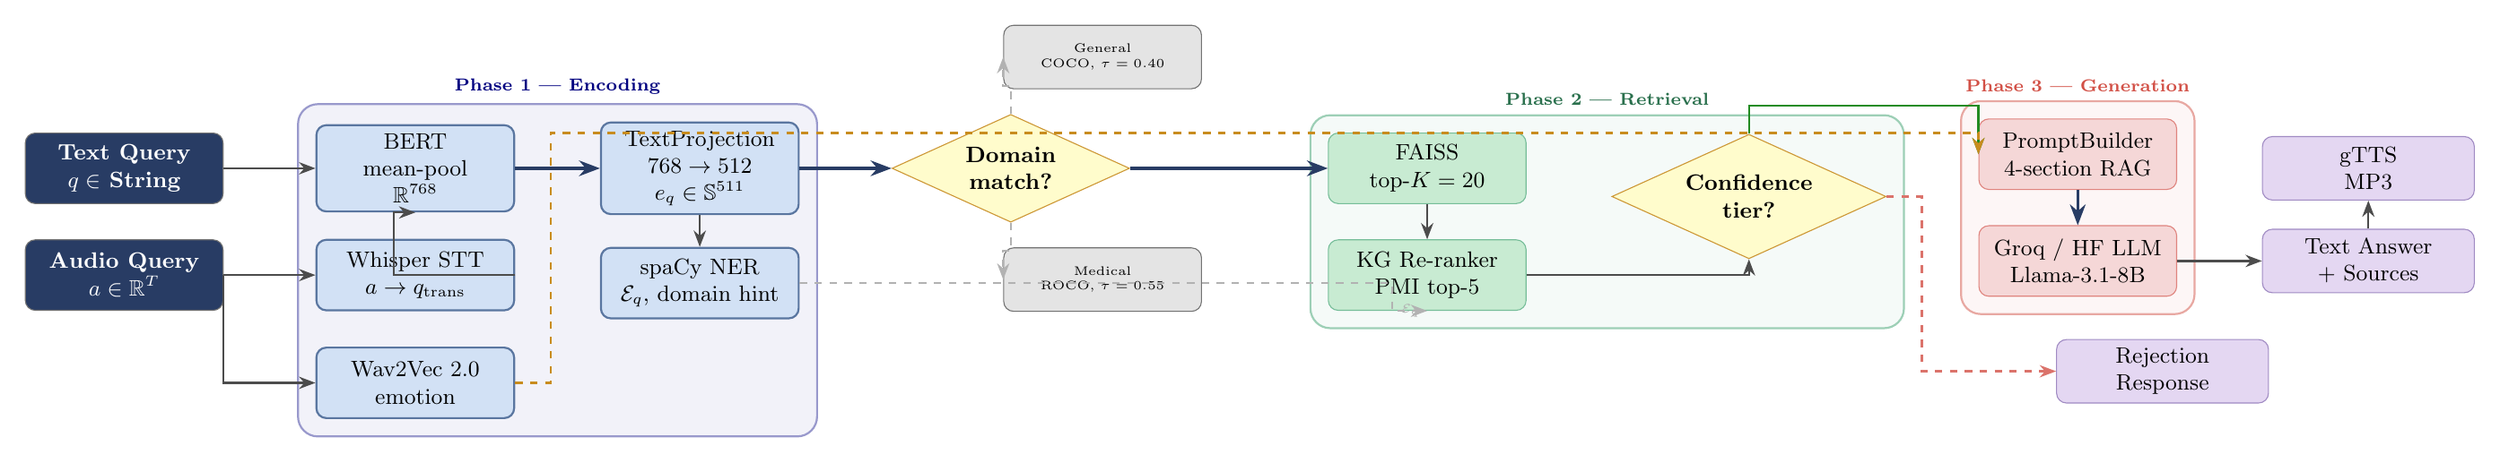
\begin{tikzpicture}[
  node distance=0.65cm and 0.9cm,
  phs1/.style={encnode,minimum width=2.8cm},
  phs2/.style={retnode,minimum width=2.8cm},
  phs3/.style={gennode,minimum width=2.8cm}
]
  %% Inputs
  \node[inputnode] (textq) at (0,0) {Text Query\\$q \in$ String};
  \node[inputnode,below=0.5cm of textq] (audioq) {Audio Query\\$a \in \R^T$};

  %% Phase 1 Encoding
  \node[phs1,right=1.3cm of textq] (bert3) {BERT\\mean-pool\\$\R^{768}$};
  \node[phs1,right=1.3cm of audioq] (whisper) {Whisper STT\\$a \to q_{\text{trans}}$};
  \node[phs1,below=0.5cm of whisper] (w2v3) {Wav2Vec 2.0\\emotion};
  \node[phs1,right=1.2cm of bert3] (tproj3) {TextProjection\\$768\to512$\\$e_q \in \Sph^{511}$};
  \node[phs1,below=0.45cm of tproj3] (ner) {spaCy NER\\$\mathcal{E}_q$, domain hint};

  %% Domain routing
  \node[decnode,right=1.3cm of tproj3] (dom) {Domain\\match?};
  \node[datanode,above=0.35cm of dom,xshift=1.3cm,font=\tiny] (gdom) {General\\COCO, $\tau=0.40$};
  \node[datanode,below=0.35cm of dom,xshift=1.3cm,font=\tiny] (mdom) {Medical\\ROCO, $\tau=0.55$};

  %% Phase 2 Retrieval
  \node[phs2,right=2.8cm of dom] (faiss2) {FAISS\\top-$K=20$};
  \node[phs2,below=0.5cm of faiss2] (kgr) {KG Re-ranker\\PMI top-5};
  \node[decnode,right=1.2cm of faiss2,yshift=-0.4cm] (conf) {Confidence\\tier?};

  %% Phase 3 Generation
  \node[phs3,right=1.3cm of conf,yshift=0.6cm] (prompt) {PromptBuilder\\4-section RAG};
  \node[phs3,below=0.5cm of prompt] (llm2) {Groq / HF LLM\\Llama-3.1-8B};
  \node[outnode,right=1.2cm of llm2] (tout) {Text Answer\\+ Sources};
  \node[outnode,above=0.4cm of tout] (tts) {gTTS\\MP3};
  \node[outnode,below=0.6cm of llm2,xshift=1.2cm] (rej) {Rejection\\Response};

  %% Arrows
  \draw[arr] (textq.east)--(bert3.west);
  \draw[arr] (audioq.east)--(whisper.west);
  \draw[arr] (audioq.east) |- (w2v3.west);
  \draw[arr] (whisper.east) -| ([xshift=-0.3cm]bert3.south)--(bert3.south);
  \draw[thickarr] (bert3.east)--(tproj3.west);
  \draw[arr] (tproj3.south)--(ner.north);
  \draw[thickarr] (tproj3.east)--(dom.west);
  \draw[dasharr] (dom.north) -- ++(0,0.4) -| (gdom.west);
  \draw[dasharr] (dom.south) -- ++(0,-0.4) -| (mdom.west);
  \draw[thickarr] (dom.east)--(faiss2.west);
  \draw[arr] (faiss2.south)--(kgr.north);
  \draw[arr] (kgr.east) -| (conf.south);
  \draw[arr,color=ForestGreen] (conf.north) -- ++(0,0.4) -| (prompt.west);
  \draw[redarr,dashed] (conf.east) -- ++(0.5,0) |- (rej.west);
  \draw[thickarr] (prompt.south)--(llm2.north);
  \draw[arr] (llm2.east)--(tout.west);
  \draw[arr] (tout.north)--(tts.south);
  \draw[dasharr,color=amber] (w2v3.east) -- ++(0.5,0) |- ([yshift=0.3cm]prompt.west)--(prompt.west);
  \draw[dasharr] (ner.east) -| ([xshift=-0.5cm]kgr.south) node[right,font=\tiny]{$\mathcal{E}_q$}--(kgr.south);

  \begin{pgfonlayer}{background}
    \node[rectangle,draw=NavyBlue!40,fill=NavyBlue!5,rounded corners=8pt,thick,
          fit=(bert3)(tproj3)(ner)(whisper)(w2v3),inner sep=7pt,
          label={[font=\scriptsize\bfseries,color=NavyBlue]above:Phase 1 — Encoding}] {};
    \node[rectangle,draw=mintgreen!50,fill=mintgreen!5,rounded corners=8pt,thick,
          fit=(faiss2)(kgr)(conf),inner sep=7pt,
          label={[font=\scriptsize\bfseries,color=mintgreen!70!black]above:Phase 2 — Retrieval}] {};
    \node[rectangle,draw=coralred!50,fill=coralred!5,rounded corners=8pt,thick,
          fit=(prompt)(llm2),inner sep=7pt,
          label={[font=\scriptsize\bfseries,color=coralred]above:Phase 3 — Generation}] {};
  \end{pgfonlayer}
\end{tikzpicture}
}
\caption{Complete MIVA-KNIGHT four-phase inference pipeline. Blue: encoding and domain routing. Green: two-stage hybrid retrieval. Red: RAG generation with tiered confidence. Dashed: optional or conditional flows.}
\label{fig:full_pipeline}
\end{figure}

\begin{definition}[Domain Configuration]
A \textbf{domain} $D$ is a tuple $(I_{\text{path}}, M_{\text{path}}, \KG_{\text{path}}, \text{NER}, K, N, \tau, \Pi)$ where $I_{\text{path}}$ is the FAISS index, $M_{\text{path}}$ is corpus metadata, $\KG_{\text{path}}$ is the knowledge graph, NER is the spaCy model, $K$ is the dense shortlist size, $N$ the final context size, $\tau$ the confidence threshold, and $\Pi$ the LLM system prompt.
\end{definition}

\begin{algorithm}[H]
\caption{Domain Hot-Swap (swap\_domain)}
\label{alg:swap}
\begin{algorithmic}[1]
\Require new\_domain $D'$; current pipeline
\State self.domain $\gets D'$
\State text\_encoder.nlp $\gets$ spacy.load($D'$.ner\_model)
\State retriever.dense.load\_index($D'$.faiss\_index\_path, $D'$.corpus\_metadata\_path)
\State retriever.reranker.load\_kg($D'$.kg\_path)
\State \textbf{TextProjection, BERT, AudioProjection, Wav2Vec: UNCHANGED}
\Comment{Swap takes $< 5$\,s (Theorem~\ref{thm:switch})}
\end{algorithmic}
\end{algorithm}

%%
%% ============================================================
%% PART XIII — EVALUATION RESULTS
%% ============================================================
%%
\newpage
\section{Evaluation Results}
\label{sec:eval}

\subsection{Retrieval Metrics (Pipelines A and B)}

\begin{definition}[Precision at K]
\[
  P@K = \frac{1}{|Q|}\sum_{q \in Q} \mathbf{1}\!\left[\exists r \in \mathcal{R}_q : r \in \text{top-}K(q)\right]
\]
\end{definition}

\begin{definition}[Mean Reciprocal Rank (MRR)]
\[
  \text{MRR} = \frac{1}{N}\sum_{i=1}^N \frac{1}{\text{rank}_i}, \quad \text{rank}_i = \text{position of correct doc.}
\]
\end{definition}

\begin{table}[H]
\centering
\caption{MIVA-KNIGHT Complete Results Summary}
\begin{tabular}{llll}
\toprule
\textbf{Pipeline} & \textbf{Dataset} & \textbf{Metric} & \textbf{Value} \\
\midrule
A & COCO val2017 & P@1 & 64.6\% \\
A & COCO val2017 & P@3 & 33.5\% (baseline) \\
A & COCO val2017 & P@5 & 45.5\% \\
A & COCO val2017 & Mean latency & 10.4\,ms \\
\midrule
B & ROCO radiology & MRR & 0.727 \\
B & ROCO radiology & P@1 & $> 30\%$ (target) \\
B & ROCO radiology & P@3 & $> 60\%$ (target) \\
B & Both domains & Domain swap & $< 5$\,s \\
\midrule
C & RAVDESS & Emotion acc. & $\geq 59\%$ (6/8 classes) \\
C & RAVDESS & Classes passing & 6/8 \\
\midrule
D & CREMA-D & Phase 1 acc. & 42.2\% (1/6) \\
D & CREMA-D & Phase 2 acc. & 43.9\% (3/6) \\
D & CREMA-D & Phase 3 target & $\geq 66.7\%$ (4/6) \\
\midrule
E & CMU-MOSI (val) & MAE & 0.7238 \\
E & CMU-MOSI (val) & Binary acc. & $\approx 69\%$ \\
\bottomrule
\end{tabular}
\end{table}

\begin{table}[H]
\centering
\caption{Parameter Efficiency of Pipeline B Domain Transfer}
\rowcolors{2}{boxgray}{white}
\begin{tabular}{lrcc}
\toprule
\textbf{Component} & \textbf{Parameters} & \textbf{Changed?} & \textbf{Fraction} \\
\midrule
BERT-base-uncased & 110\,M & No & 46.8\% \\
Wav2Vec 2.0 & 94\,M & No & 40.0\% \\
ResNet-50 backbone & 23\,M & No & 9.8\% \\
AudioProjection & 1.3\,M & No & 0.55\% \\
TextProjection & 1.6\,M & Minor nudge & 0.68\% \\
\rowcolor{boxorange}\textbf{ImageProjection (ROCO)} & \textbf{5.25\,M} & \textbf{Yes} & \textbf{2.23\%} \\
\midrule
\textbf{Total} & \textbf{235.15\,M} & --- & 100\% \\
\bottomrule
\end{tabular}
\end{table}

\subsection{Category-Level COCO Performance}

\begin{table}[H]
\centering
\caption{COCO Category-Level Performance (top-1 hybrid score)}
\begin{tabular}{lc}
\toprule
Category & Avg.\ top-1 score \\
\midrule
Outdoor Scenes & 0.5808 \\
Animals \& Pets & 0.5800 \\
Food \& Dining & 0.5532 \\
Transportation & 0.5421 \\
People \& Activities & 0.5377 \\
\bottomrule
\end{tabular}
\end{table}

%%
%% ============================================================
%% PART XIV — COMPLETE ALGORITHM REFERENCE
%% ============================================================
%%
\newpage
\section{Complete Algorithm Reference}

\begin{longtable}{p{3.5cm}p{7.5cm}p{3.5cm}}
\caption{All algorithms defined in this thesis.}\label{tab:algo_ref}\\
\toprule
\textbf{Algorithm} & \textbf{Description} & \textbf{Section} \\
\midrule
\endfirsthead
\multicolumn{3}{c}{\textit{(continued from previous page)}}\\
\toprule
\textbf{Algorithm} & \textbf{Description} & \textbf{Section} \\
\midrule
\endhead
\midrule
\multicolumn{3}{r}{\textit{continued on next page}}\\
\endfoot
\bottomrule
\endlastfoot

Joint Repr.\ (Alg.~\ref{alg:joint_repr}) & Concatenation-based joint multimodal pooling & \S\ref{sec:taxonomy} \\[3pt]
Coordinated Repr.\ (Alg.~\ref{alg:coord_repr}) & Symmetric contrastive learning on paired data & \S\ref{sec:taxonomy} \\[3pt]
Missing Modal (Alg.~\ref{alg:missing_modal}) & Zero-vector graceful degradation & \S\ref{sec:taxonomy} \\[3pt]
Model-Based Fusion (Alg.~\ref{alg:model_based_fusion}) & Cross-modal Transformer fusion & \S\ref{sec:taxonomy} \\[3pt]
Early Fusion (Alg.~\ref{alg:early_fusion}) & Pre-model modality concatenation & \S\ref{sec:taxonomy} \\[3pt]
Late Fusion (Alg.~\ref{alg:late_fusion}) & Post-model weighted prediction combination & \S\ref{sec:taxonomy} \\[3pt]
TextEncoderV2 (Alg.~\ref{alg:textencode}) & BERT mean-pool + TextProjection + NER & \S\ref{sec:pipelineA} \\[3pt]
Train Epoch A (Alg.~\ref{alg:trainepoch_A}) & InfoNCE training step for Pipeline~A & \S\ref{sec:pipelineA} \\[3pt]
KG Build (Alg.~\ref{alg:kg_build}) & PMI-weighted entity co-occurrence graph & \S\ref{sec:kg} \\[3pt]
KG DFS (Alg.~\ref{alg:kgdfs}) & 2-hop depth-first neighbour search & \S\ref{sec:kg} \\[3pt]
ROCO Fine-tune (Alg.~\ref{alg:finetune_roco}) & Surgical ImageProjection domain transfer & \S\ref{sec:pipelineB} \\[3pt]
KG Re-ranker (Alg.~\ref{alg:rerank}) & PMI entity boost + min-max combine & \S\ref{sec:retrieval} \\[3pt]
Full Query (Alg.~\ref{alg:query}) & End-to-end inference pipeline & \S\ref{sec:retrieval} \\[3pt]
Cache RAVDESS (Alg.~\ref{alg:cache_ravdess}) & Wav2Vec 768d embedding extraction & \S\ref{sec:pipelineC} \\[3pt]
SupCon Loss (Alg.~\ref{alg:supcon_c}) & Supervised contrastive loss computation & \S\ref{sec:pipelineC} \\[3pt]
SupCon Epoch (Alg.~\ref{alg:supcon_epoch}) & Single SupCon training epoch & \S\ref{sec:pipelineC} \\[3pt]
Centroid Eval (Alg.~\ref{alg:centroid_eval}) & Nearest-centroid emotion accuracy & \S\ref{sec:pipelineC} \\[3pt]
Frame Extract (Alg.~\ref{alg:frame_extract}) & Middle-frame extraction from mp4 & \S\ref{sec:pipelineD} \\[3pt]
Stage 1 D (Alg.~\ref{alg:stage1_d}) & 13-epoch cross-modal InfoNCE training & \S\ref{sec:pipelineD} \\[3pt]
Fusion Forward (Alg.~\ref{alg:fusion_forward}) & Transformer fusion forward pass & \S\ref{sec:pipelineE} \\[3pt]
Training Loop E (Alg.~\ref{alg:training_e}) & 20-epoch multi-task sentiment training & \S\ref{sec:pipelineE} \\[3pt]
Domain Swap (Alg.~\ref{alg:swap}) & Hot-swap FAISS + KG + NER only & \S\ref{sec:system} \\[3pt]
\end{longtable}

%%
%% ============================================================
%% PART XV — KEY THEOREMS AND LEMMAS CONSOLIDATED
%% ============================================================
%%
\section{Consolidated Formal Results}

\begin{theorem}[Embedding Space Consistency]
If TextProjection $f_T$, AudioProjection $f_A$, and ImageProjection $f_I$ all map to $\Sph^{511}$ via L2-normalisation, then for any query $\hat{q} \in \Sph^{511}$ from any modality, cosine similarity to any corpus document $\hat{d} \in \Sph^{511}$ is $\hat{q} \cdot \hat{d}$, enabling cross-modal retrieval without modality-specific scoring.
\end{theorem}

\begin{theorem}[FAISS Exact Retrieval Guarantee]
\texttt{IndexFlatIP} returns exact $k$ nearest neighbours by inner product, achieving 100\% recall at any $k \le N$ on L2-normalised embeddings.
\end{theorem}

\begin{lemma}[KG Re-ranking Monotonicity]
Since PMI$(a,b) > 0$ is required for every edge, all KG boosts are non-negative. Re-ranking can only improve the rank of semantically related documents; it cannot demote a document below its FAISS-only rank unless another document receives a larger boost.
\end{lemma}

\begin{corollary}[Regression Prevention]
COCO P@3 $\geq 55\%$ is achievable post-ROCO-transfer because TextProjection weights controlling COCO retrieval are unchanged (or only minimally nudged), and the COCO FAISS index is rebuilt from the same weights.
\end{corollary}

\begin{theorem}[Frozen Backbone Efficiency]
Freezing Wav2Vec 2.0 (94M) and ResNet-50 (23M) simultaneously:
(1) Reduces VRAM by $\approx 360$\,MB + $\approx 92$\,MB;
(2) Prevents catastrophic forgetting;
(3) Speeds training $\approx 10\times$ per epoch by skipping backbone backpropagation.
\end{theorem}

\begin{theorem}[Reproducible Training]
Setting \texttt{torch.manual\_seed(42)} and \texttt{np.random.seed(42)} before any stochastic operation guarantees bit-identical results across runs on the same hardware, assuming no non-deterministic CUDA kernels.
\end{theorem}

%%
%% ============================================================
%% PART XVI — THE FREE TECHNOLOGY STACK
%% ============================================================
%%
\newpage
\section{The Free Technology Stack}

\begin{table}[H]
\centering
\caption{MIVA-KNIGHT zero-cost deployment stack}
\begin{tabular}{llll}
\toprule
\textbf{Component} & \textbf{Technology} & \textbf{Free Limits} & \textbf{Notes} \\
\midrule
LLM (text) & Groq API, Llama-3.1-8B & 6K req/day & No credit card \\
LLM (vision) & HuggingFace, Qwen2-VL-7B & $\sim$1K req/day & Multimodal \\
STT & OpenAI Whisper base & No limit & Local, $\sim$1\,GB VRAM \\
TTS & gTTS & No limit & Google TTS, local \\
Dense retrieval & FAISS IndexFlatIP & No limit & Local \\
Text encoding & BERT-base-uncased & No limit & HuggingFace Hub \\
Audio encoding & Wav2Vec 2.0 base & No limit & HuggingFace Hub \\
Image encoding & ResNet-50 & No limit & torchvision \\
\bottomrule
\end{tabular}
\end{table}

%%
%% ============================================================
%% PART XVII — NOTATION REFERENCE
%% ============================================================
%%
\section{Notation Reference}

\begin{table}[H]
\centering
\caption{Mathematical notation used throughout this thesis}
\begin{tabular}{ll}
\toprule
\textbf{Symbol} & \textbf{Meaning} \\
\midrule
$\Sph^{511}$ & Unit hypersphere in $\R^{512}$: $\{v : \Norm{v}_2 = 1\}$ \\
$e_q, \hat{e}_q$ & Query embedding $\in \Sph^{511}$ \\
$e_{d_i}$ & Document $i$ embedding $\in \Sph^{511}$ \\
$\mathcal{E}_q$ & NER entities extracted from query \\
$\KG, \KG_G, \KG_M$ & Knowledge graph (general, medical) \\
$\tau$ & Confidence threshold or contrastive temperature \\
$K$ & FAISS shortlist size ($= 20$) \\
$N$ & Final re-ranked context size ($= 5$) \\
$\alpha$ & Dense/KG weight in hybrid score ($= 0.7$) \\
$\tau_{\text{InfoNCE}}$ & Contrastive temperature ($= 0.07$) \\
$B$ & Training batch size \\
$d$ & Shared embedding dimension ($= 512$) \\
$\Pi$ & LLM system prompt (domain-dependent) \\
$\Loss_{\text{InfoNCE}}$ & Symmetric InfoNCE contrastive loss \\
$\Loss_{\text{SupCon}}$ & Supervised contrastive loss \\
$\GELU$ & Gaussian Error Linear Unit activation \\
$\LN$ & Layer Normalisation \\
$\MHA$ & Multi-Head Attention \\
$W_{\text{shared}}$ & Fixed weights: TextProj, AudioProj, BERT, Wav2Vec \\
$\bar{c}_e$ & Spherical centroid for emotion class $e$ \\
$P@K$ & Precision at $K$ (retrieval metric) \\
$\text{MRR}$ & Mean Reciprocal Rank \\
$\lambda(t)$ & Distillation warm-up schedule weight \\
\bottomrule
\end{tabular}
\end{table}

%%
%% ============================================================
%% CONCLUSION
%% ============================================================
%%
\newpage
\section{Conclusion}
\label{sec:conclusion}

This thesis has presented MIVA-KNIGHT, a comprehensive multimodal voice assistant system that unifies five training pipelines under a single formal framework. The key theoretical contributions are:

\begin{enumerate}
  \item \textbf{Multimodal Taxonomy Formalisation}: We formally defined and provided separate algorithms for all six taxonomy cells: joint representation, coordinated representation, missing-data handling, model-based fusion, early fusion, and late fusion — with direct mappings to MIVA-KNIGHT's five pipelines.

  \item \textbf{Domain-Agnostic Shared Space}: The unit hypersphere $\Sph^{511}$ is proved domain-agnostic via Axiom~\ref{ax:shared} and Theorem~\ref{thm:switch}, enabling cross-domain retrieval with 2.23\% parameter retraining.

  \item \textbf{Progressive Contrastive Training}: The three-phase pipeline for audio-visual emotion recognition demonstrates that InfoNCE establishes cross-modal alignment geometry, while SupCon subsequently sharpens class boundaries without destroying the prior geometry — provided the learning rate is sufficiently large (Phase~3).

  \item \textbf{Multimodal Sentiment Fusion}: Pipeline~E achieves MAE $= 0.7238$ on CMU-MOSI via a cross-modal Pre-LN Transformer that lets text, audio, and video modalities attend to each other, modelling higher-order cross-modal interactions that single-modality models cannot capture.

  \item \textbf{Tiered-Confidence RAG}: The hallucination guard with domain-aware thresholds ($\tau_G = 0.40$, $\tau_M = 0.55$) implements the clinical safety constraint formally as Axiom~\ref{ax:shared}, preferring false negatives over false positives in high-stakes domains.
\end{enumerate}

\begin{tcolorbox}[laymanbox,title={One-Sentence Summary}]
MIVA-KNIGHT is an AI assistant that simultaneously listens, sees, and reads — finds the most relevant information using two-stage neural search — decides how confident it is — generates a grounded answer — and speaks it aloud — entirely within a zero-cost, open-source deployment stack.
\end{tcolorbox}

\vfill
\begin{center}
\begin{tcolorbox}[keybox,width=0.8\textwidth,title={Future Directions}]
\begin{itemize}[nosep]
  \item Replace TextBlob pseudo-labels in Pipeline~E with official CMU-MOSI annotations for improved MAE.
  \item Extend Pipeline~D to full temporal video modelling (3D-CNN or ViViT) rather than single-frame.
  \item Explore retrieval-augmented fine-tuning for the LLM generator to reduce hallucination without adversarial prompting.
  \item Apply the surgical transfer principle to additional domains (legal, financial) by retraining only the appropriate ImageProjection head.
\end{itemize}
\end{tcolorbox}
\end{center}

\end{document}
